%% Empirical Evaluation of a Build-Graph-First, Deterministic
%% Fact-Extraction -> Structurizr Architecture Pipeline
%% Target: SANER 2027 Research Track (IEEE format).
%% See ../plans/2026-06-04-empirical-evaluation-fact-extraction-pipeline.md
%%
%% BUILD: `make` (latexmk) in this directory. Tables/figures/macros under
%% tables/, figures/, generated/ are GENERATED from raw experiment data by the
%% analysis/ pipeline (see README.md, plan section 15) -- do not hand-edit them.

%% SANER 2027 requires exactly this: 10pt, conference, no compsoc/compsocconf.
\documentclass[10pt,conference]{IEEEtran}
\IEEEoverridecommandlockouts

% --- packages ---
\usepackage{cite}
\usepackage{amsmath,amssymb,amsfonts}
\usepackage{graphicx}
\usepackage{booktabs}      % generated tables use \toprule/\midrule/\bottomrule
\usepackage{siunitx}       % aligned numbers in generated tables
\usepackage{xcolor}
\usepackage{tikz}          % figures emitted as .pgf by analysis/make_figures.py are tikzpictures
\usepackage{url}
%% NOT microtype: it is not installed and MiKTeX's auto-install hangs on this machine (memory
%% latex-toolchain-setup); the page budget is met by content, not by font expansion.
\usepackage[hidelinks]{hyperref}

\graphicspath{{figures/}}

%% SANER 2027 enforces full double-anonymous review: a submission carrying author
%% names, affiliations, or acknowledgments is desk-rejected without review.
%% Keep this TRUE for the 25 Sep 2026 submission build; flip to \anonymousfalse
%% for internal drafts and for the camera-ready (notification 1 Dec 2026).
\newif\ifanonymous
\anonymoustrue

%% Eval plan section 1.4 #5: the SANER manuscript ALSO anonymizes the TOOL, not just the
%% authors -- the CFP requires that the submission not be trivially associable with a
%% public version, and the technical report is the artifact that carries the real name.
%% Prose therefore NEVER writes the tool name literally: use \tool, which resolves to the real
%% name only in the non-anonymous build. The console-script name `arch` is generic, is not
%% in the anonymity audit list, and is what the artifact's README and pyproject install in
%% both builds -- so \cli is `arch` everywhere (audit 2026-08-31: the anonymous PDF said
%% `anon propose` while the artifact shipped `arch`).
\ifanonymous
  \newcommand{\tool}{\textsc{Anon}}
  \newcommand{\cli}{\texttt{arch}}
\else
  \newcommand{\tool}{\textsc{Anon}}
  \newcommand{\cli}{\texttt{arch}}
\fi

%% Bibliography scaffold switch. \nocite{*} typesets every references.bib entry; it was the
%% build-green scaffold while section II was a placeholder. OFF since 2026-08-30 (section II
%% cites for real; every entry verified). A SUBMISSION MUST NOT LIST UNCITED REFERENCES --
%% keep this false and verify the reference list before 25 Sep 2026.
\newif\ifdraftbib
\draftbibfalse   % Section II cites for real since 2026-08-30; uncited references.bib entries stay out of the list

%% Companion technical report (response plan section 13, 2026-09-13). The paper is
%% self-contained on every claim; procedures, sensitivity analyses, and per-system tables live in
%% the anonymized TR shipped in the mirror package (latex/tr.tex, built from the SAME macros and
%% tables). Forward references are macros so a TR reorder is a one-line fix here.
\newcommand{\TR}{TR}
\newcommand{\trExtract}{\TR{}\,\S2}      % evidence extraction per build idiom
\newcommand{\trInputs}{\TR{}\,\S3}       % baseline inputs, entity ownership, LLM runner
\newcommand{\trStats}{\TR{}\,\S4}        % metrics and inferential procedures, full p-values
\newcommand{\trDiagnostic}{\TR{}\,\S5}   % reference-free diagnostic: sensitivity, Tier-B calls
\newcommand{\trPublished}{\TR{}\,\S6}    % published scores on shared references (SARIF, FCA)
\newcommand{\trAblation}{\TR{}\,\S7}     % ablation detail (A1 per layer, A3/A4)
\newcommand{\trDrift}{\TR{}\,\S8}        % drift arms: per-operator, combined-loss, history tables
\newcommand{\trPerf}{\TR{}\,\S9}         % per-system performance table
\newcommand{\trCuration}{\TR{}\,\S10}    % blind curation: rater agreement, effort table

% --- generated numbers: every in-prose statistic is a \newcommand here, ---
% --- emitted by analysis/make_macros.py. Prose cites macros, never literals. ---
%% GENERATED by analysis/make_macros.py -- DO NOT EDIT BY HAND.
%% Refreshing the data re-typesets the paper (plan §15).
\newcommand{\corpusCppCount}{5}
\newcommand{\corpusCsCount}{4}
\newcommand{\corpusReferenceCount}{9}
\newcommand{\corpusSystemCount}{9}
\newcommand{\rqAdequacyAdequateCount}{4}
\newcommand{\rqAdequacyCppLargestMax}{0.3028}
\newcommand{\rqAdequacyCppRatioMax}{0.1306}
\newcommand{\rqAdequacyFmtEntities}{66}
\newcommand{\rqAdequacyFmtLargest}{0.3182}
\newcommand{\rqAdequacyFmtRatio}{0.3333}
\newcommand{\rqAdequacyFmtUnits}{22}
\newcommand{\rqAdequacyInadequateCount}{5}
\newcommand{\rqAdequacyLargestIntervalHi}{0.7759}
\newcommand{\rqAdequacyLargestIntervalLo}{0.3028}
\newcommand{\rqAdequacyLargestMax}{0.5}
\newcommand{\rqAdequacyLibxmlLargestShare}{0.7759}
\newcommand{\rqAdequacyLibxmlRatio}{0.2414}
\newcommand{\rqAdequacyLooCorrect}{8/9}
\newcommand{\rqAdequacyLooLargestClauseFolds}{0}
\newcommand{\rqAdequacyLooWrong}{libxml2}
\newcommand{\rqAdequacyN}{9}
\newcommand{\rqAdequacyRatioIntervalHi}{1.0}
\newcommand{\rqAdequacyRatioIntervalLo}{0.1306}
\newcommand{\rqAdequacyRatioMax}{0.25}
\newcommand{\rqAdequacyRatioOnlyHiSystem}{libxml2}
\newcommand{\rqAdequacyRatioOnlyIntervalHi}{0.2414}
\newcommand{\rqAdequacyRhoBootReps}{2000}
\newcommand{\rqAdequacyRhoCiHi}{-0.093}
\newcommand{\rqAdequacyRhoCiLo}{-0.982}
\newcommand{\rqAdequacyRhoMqMoJo}{0.696}
\newcommand{\rqAdequacyRhoRatioAtoA}{-0.583}
\newcommand{\rqAdequacyRhoRatioMoJo}{-0.766}
\newcommand{\rqAdequacyRuleAgreement}{9/9}
\newcommand{\rqAdequacySerilogEntities}{6}
\newcommand{\rqAdequacySerilogLargest}{0.1667}
\newcommand{\rqAdequacySerilogRatio}{1.0}
\newcommand{\rqAdequacySerilogUnits}{6}
\newcommand{\rqAdequacyTerminalEntities}{63}
\newcommand{\rqAdequacyTerminalLargest}{0.0159}
\newcommand{\rqAdequacyTerminalRatio}{1.0}
\newcommand{\rqAdequacyTerminalUnits}{63}
\newcommand{\rqAdequacyTierBAdequateList}{none}
\newcommand{\rqAdequacyTierBInadequateList}{fmt, Serilog, Terminal}
\newcommand{\rqAdequacyTierBSystems}{3}
\newcommand{\rqFiveAcdcChurnMedian}{74.8}
\newcommand{\rqFiveAcdcChurnWorst}{47.7}
\newcommand{\rqFiveDirChurnMedian}{100.0}
\newcommand{\rqFivePipelineChurn}{100.0}
\newcommand{\rqNineEshopAri}{0.527}
\newcommand{\rqNineEshopBestSarAtoA}{85.87}
\newcommand{\rqNineEshopBestSarMoJo}{26.67}
\newcommand{\rqNineEshopBestSarName}{LIMBO}
\newcommand{\rqNineEshopConsensusClusters}{14.0}
\newcommand{\rqNineEshopCuratorAtoA}{95.79}
\newcommand{\rqNineEshopCuratorAtoASpread}{4.97}
\newcommand{\rqNineEshopCuratorClusters}{10.0}
\newcommand{\rqNineEshopCuratorCode}{R-A}
\newcommand{\rqNineEshopCuratorCount}{2}
\newcommand{\rqNineEshopCuratorEdgeFone}{0.629}
\newcommand{\rqNineEshopCuratorEdgeFoneSpread}{0.07}
\newcommand{\rqNineEshopCuratorFullRefAtoA}{TBD}
\newcommand{\rqNineEshopCuratorFullRefMoJo}{TBD}
\newcommand{\rqNineEshopCuratorMinusRatersMoJo}{20.15}
\newcommand{\rqNineEshopCuratorMoJo}{86.67}
\newcommand{\rqNineEshopCuratorMoJoSpread}{20.0}
\newcommand{\rqNineEshopCuratorPairAri}{0.747}
\newcommand{\rqNineEshopCuratorPairAtoA}{93.94}
\newcommand{\rqNineEshopCuratorPairKappaAligned}{0.824}
\newcommand{\rqNineEshopCuratorPairMoJo}{80.62}
\newcommand{\rqNineEshopCuratorPairNmi}{0.943}
\newcommand{\rqNineEshopCuratorVsConsensusAtoA}{92.0}
\newcommand{\rqNineEshopCuratorVsConsensusMoJo}{75.0}
\newcommand{\rqNineEshopFloorAtoA}{80.77}
\newcommand{\rqNineEshopFloorMoJo}{33.33}
\newcommand{\rqNineEshopGroups}{11.0}
\newcommand{\rqNineEshopKappa}{0.0}
\newcommand{\rqNineEshopKappaAligned}{0.702}
\newcommand{\rqNineEshopLabelsShared}{0}
\newcommand{\rqNineEshopLeakageDelta}{20.0}
\newcommand{\rqNineEshopMinutes}{43}
\newcommand{\rqNineEshopNmi}{0.868}
\newcommand{\rqNineEshopNonBlindMoJo}{66.67}
\newcommand{\rqNineEshopOps}{43.0}
\newcommand{\rqNineEshopOverBestSarMoJo}{60.0}
\newcommand{\rqNineEshopOverFloorMoJo}{53.34}
\newcommand{\rqNineEshopPairAgreement}{0.918}
\newcommand{\rqNineEshopProposeDerivedPct}{0}
\newcommand{\rqNineEshopRaterConflicts}{0}
\newcommand{\rqNineEshopRaterPairAtoA}{89.69}
\newcommand{\rqNineEshopRaterPairMoJo}{66.52}
\newcommand{\rqNineEshopRaterRefAriMin}{0.615}
\newcommand{\rqNineEshopRaterRefKappaAlignedMax}{0.937}
\newcommand{\rqNineEshopRaterRefKappaAlignedMin}{0.762}
\newcommand{\rqNineEshopRaterRefKappaMin}{0.0}
\newcommand{\rqNineEshopRaterRefMoJoMin}{74.16}
\newcommand{\rqNineEshopRaterRefNmiMin}{0.901}
\newcommand{\rqNineEshopRuleLines}{63.0}
\newcommand{\rqNineEshopSecondCuratorAtoA}{90.82}
\newcommand{\rqNineEshopSecondCuratorCode}{R-B}
\newcommand{\rqNineEshopSecondCuratorEdgeFone}{0.564}
\newcommand{\rqNineEshopSecondCuratorMinutes}{120}
\newcommand{\rqNineEshopSecondCuratorMoJo}{66.67}
\newcommand{\rqNineEshopSecondCuratorOps}{36.0}
\newcommand{\rqNineMedianCuratorMinusRatersMoJo}{17.8}
\newcommand{\rqNineSquidexAri}{0.228}
\newcommand{\rqNineSquidexBestSarAtoA}{92.96}
\newcommand{\rqNineSquidexBestSarMoJo}{60.0}
\newcommand{\rqNineSquidexBestSarName}{LIMBO}
\newcommand{\rqNineSquidexConsensusClusters}{12.0}
\newcommand{\rqNineSquidexCuratorAtoA}{95.83}
\newcommand{\rqNineSquidexCuratorClusters}{13.0}
\newcommand{\rqNineSquidexCuratorCode}{R-C}
\newcommand{\rqNineSquidexCuratorCount}{1}
\newcommand{\rqNineSquidexCuratorEdgeFone}{0.667}
\newcommand{\rqNineSquidexCuratorFullRefAtoA}{96.43}
\newcommand{\rqNineSquidexCuratorFullRefMoJo}{75.0}
\newcommand{\rqNineSquidexCuratorMinusRatersMoJo}{15.45}
\newcommand{\rqNineSquidexCuratorMoJo}{70.0}
\newcommand{\rqNineSquidexFloorAtoA}{92.0}
\newcommand{\rqNineSquidexFloorMoJo}{70.0}
\newcommand{\rqNineSquidexGroups}{12.0}
\newcommand{\rqNineSquidexKappa}{0.391}
\newcommand{\rqNineSquidexKappaAligned}{0.586}
\newcommand{\rqNineSquidexLabelsShared}{4}
\newcommand{\rqNineSquidexMinutes}{210}
\newcommand{\rqNineSquidexNmi}{0.766}
\newcommand{\rqNineSquidexOps}{46.0}
\newcommand{\rqNineSquidexOverBestSarMoJo}{10.0}
\newcommand{\rqNineSquidexOverFloorMoJo}{0.0}
\newcommand{\rqNineSquidexPairAgreement}{0.78}
\newcommand{\rqNineSquidexProposeDerivedPct}{0}
\newcommand{\rqNineSquidexRaterConflicts}{0}
\newcommand{\rqNineSquidexRaterPairAtoA}{86.3}
\newcommand{\rqNineSquidexRaterPairMoJo}{54.55}
\newcommand{\rqNineSquidexRaterRefAriMin}{n/a}
\newcommand{\rqNineSquidexRaterRefKappaAlignedMax}{n/a}
\newcommand{\rqNineSquidexRaterRefKappaAlignedMin}{n/a}
\newcommand{\rqNineSquidexRaterRefKappaMin}{n/a}
\newcommand{\rqNineSquidexRaterRefMoJoMin}{n/a}
\newcommand{\rqNineSquidexRaterRefNmiMin}{n/a}
\newcommand{\rqNineSquidexRuleLines}{59.0}
\newcommand{\rqNineSystems}{2}
\newcommand{\rqNineSystemsWithTwoCurators}{1}
\newcommand{\rqNineTwoCuratorSystemsList}{eShop}
\newcommand{\rqOneFloorAbseilAri}{44.06}
\newcommand{\rqOneFloorAbseilNested}{100.0}
\newcommand{\rqOneFloorAdequateAri}{64.88}
\newcommand{\rqOneFloorAdequateAtoA}{91.39}
\newcommand{\rqOneFloorAdequateMoJo}{94.4}
\newcommand{\rqOneFloorBashAri}{85.69}
\newcommand{\rqOneFloorCppAri}{44.06}
\newcommand{\rqOneFloorCppAtoA}{85.13}
\newcommand{\rqOneFloorCppMoJo}{91.94}
\newcommand{\rqOneFloorCsAri}{0.0}
\newcommand{\rqOneFloorCsAtoA}{80.48}
\newcommand{\rqOneFloorCsMoJo}{35.41}
\newcommand{\rqOneFloorItkAri}{22.61}
\newcommand{\rqOneFloorItkAtoA}{84.21}
\newcommand{\rqOneFloorItkNested}{96.15}
\newcommand{\rqOneFloorOpencvAri}{100.0}
\newcommand{\rqOneLlmEshopMoJo}{86.67}
\newcommand{\rqOneMedianAri}{84.07}
\newcommand{\rqOneMedianAtoA}{95.83}
\newcommand{\rqOneMedianMoJo}{72.11}
\newcommand{\rqOneProposeAbseilAri}{100.0}
\newcommand{\rqOneProposeAbseilMoJo}{100.0}
\newcommand{\rqOneProposeAdequateAri}{78.78}
\newcommand{\rqOneProposeCppMoJo}{82.66}
\newcommand{\rqOneProposeCsMoJo}{59.73}
\newcommand{\rqOneProposeEshopMoJo}{0.0}
\newcommand{\rqOneProposeItkAri}{84.6}
\newcommand{\rqOneProposeMedianMoJo}{69.47}
\newcommand{\rqOneProposeOpencvMoJo}{48.29}
\newcommand{\rqSevenColdBudget}{11/12}
\newcommand{\rqSevenItkClangSharePct}{1.5}
\newcommand{\rqSevenItkCmakeSharePct}{3.4}
\newcommand{\rqSevenItkColdMin}{410.0}
\newcommand{\rqSevenItkDoxygenSharePct}{93.4}
\newcommand{\rqSevenItkLZeroImpliedMin}{20.9}
\newcommand{\rqSevenItkWarmMin}{9.1}
\newcommand{\rqSevenMaxColdMin}{410.0}
\newcommand{\rqSevenMaxKloc}{825}
\newcommand{\rqSevenMaxPeakRssGb}{1.6}
\newcommand{\rqSevenMedianSpeedup}{4.28}
\newcommand{\rqSevenMinKloc}{0.1}
\newcommand{\rqSevenScalingSlope}{0.554}
\newcommand{\rqSevenSystems}{12}
\newcommand{\rqSevenWarmBudget}{10/12}
\newcommand{\rqSixAliasSurvival}{16/16}
\newcommand{\rqSixCombFindings}{458}
\newcommand{\rqSixCombFpTotal}{0}
\newcommand{\rqSixCombLoseLZeroAdvisory}{36}
\newcommand{\rqSixCombLoseLZeroDrift}{0}
\newcommand{\rqSixCombLoseLZeroGap}{422}
\newcommand{\rqSixCombLoseLZeroSilent}{0}
\newcommand{\rqSixCombModes}{4}
\newcommand{\rqSixCombMutations}{95}
\newcommand{\rqSixCombPrefixSilentOps}{add\_target, rename\_target}
\newcommand{\rqSixCombPrefixSilentTotal}{36}
\newcommand{\rqSixCombSilentModes}{none}
\newcommand{\rqSixCombSilentOps}{none}
\newcommand{\rqSixCombSilentTotal}{0}
\newcommand{\rqSixCombStarveMutatedAdvisory}{117}
\newcommand{\rqSixCombStarveMutatedDrift}{99}
\newcommand{\rqSixCombStarveMutatedGap}{242}
\newcommand{\rqSixCombStarveMutatedSilent}{0}
\newcommand{\rqSixCombStarveTenAdvisory}{31}
\newcommand{\rqSixCombStarveTenDrift}{404}
\newcommand{\rqSixCombStarveTenGap}{23}
\newcommand{\rqSixCombStarveTenSilent}{0}
\newcommand{\rqSixCombStarveThirtyAdvisory}{80}
\newcommand{\rqSixCombStarveThirtyDrift}{301}
\newcommand{\rqSixCombStarveThirtyGap}{77}
\newcommand{\rqSixCombStarveThirtySilent}{0}
\newcommand{\rqSixCombSystems}{5}
\newcommand{\rqSixDegradationSystems}{8}
\newcommand{\rqSixFOne}{1.0}
\newcommand{\rqSixFpPerPr}{0.0}
\newcommand{\rqSixHistArchitectural}{14}
\newcommand{\rqSixHistBuildCommits}{247}
\newcommand{\rqSixHistCommits}{1633}
\newcommand{\rqSixHistCoverageGaps}{0}
\newcommand{\rqSixHistFindings}{26}
\newcommand{\rqSixHistLabelsAgree}{25/26}
\newcommand{\rqSixHistLabelsKappa}{0.922}
\newcommand{\rqSixHistLabelsPending}{done}
\newcommand{\rqSixHistNewTargets}{9}
\newcommand{\rqSixHistNewUnmapped}{0}
\newcommand{\rqSixHistNoise}{0}
\newcommand{\rqSixHistNonArchitectural}{11}
\newcommand{\rqSixHistPairs}{8}
\newcommand{\rqSixHistPairsZero}{3}
\newcommand{\rqSixHistPairsZeroBuildChurn}{3}
\newcommand{\rqSixHistSystems}{3}
\newcommand{\rqSixMcNemarP}{\ensuremath{<}0.0001}
\newcommand{\rqSixMutationCount}{95}
\newcommand{\rqSixMutationSystems}{5}
\newcommand{\rqSixMutationsDetected}{95/95}
\newcommand{\rqSixOperatorCount}{6}
\newcommand{\rqSixPrecision}{1.0}
\newcommand{\rqSixRecall}{1.0}
\newcommand{\rqSixRenameAccuracy}{1.0}
\newcommand{\rqSixSuppressionRate}{1.0}
\newcommand{\rqSixWouldBeFalse}{5409}
\newcommand{\rqThreeAfiveEshopEdgesSaved}{30}
\newcommand{\rqThreeAfiveEshopRefRecallDrop}{1.0}
\newcommand{\rqThreeAfiveEshopRefRecallDropOperating}{0.0}
\newcommand{\rqThreeAfiveOperatingEdgesSaved}{0}
\newcommand{\rqThreeAfiveOperatingRankBiserial}{n/a}
\newcommand{\rqThreeAfiveOperatingSystemsChecked}{8}
\newcommand{\rqThreeAfiveOperatingSystemsMoved}{0}
\newcommand{\rqThreeAfiveRankBiserial}{1.0}
\newcommand{\rqThreeAfiveRefRecallDropList}{eShop 1.0, OrchardCore 0.41, nopCommerce 0.02}
\newcommand{\rqThreeAfiveRefRecallSystems}{3}
\newcommand{\rqThreeAfiveWilcoxonN}{7}
\newcommand{\rqThreeAfiveWilcoxonP}{0.0156}
\newcommand{\rqThreeCurationLiftCpp}{1.21}
\newcommand{\rqThreeCurationLiftCs}{33.86}
\newcommand{\rqThreeCurationRankBiserialAll}{1.0}
\newcommand{\rqThreeCurationRankBiserialCs}{1.0}
\newcommand{\rqThreeCurationWilcoxonP}{0.0312}
\newcommand{\rqThreeFloorCliffsCppVsCs}{0.6}
\newcommand{\rqThreeFloorCppMoJo}{92.31}
\newcommand{\rqThreeFloorCsMoJo}{35.41}
\newcommand{\rqThreeSevenMaxStructuralDelta}{0.0}
\newcommand{\rqThreeSevenSystemsChecked}{8}
\newcommand{\rqThreeSixLlmGtPipeline}{4}
\newcommand{\rqThreeSixLlmGtPipelineList}{abseil, eShop, libxml2, Squidex}
\newcommand{\rqThreeSixLlmMedianMoJo}{80.09}
\newcommand{\rqThreeSixLlmSystemsRan}{8}
\newcommand{\rqThreeSixPipelineGeLlm}{4/8}
\newcommand{\rqTwoAcdcMoJo}{28.12}
\newcommand{\rqTwoArcCsMoJo}{45.38}
\newcommand{\rqTwoArcMoJo}{36.92}
\newcommand{\rqTwoBaselineCount}{6}
\newcommand{\rqTwoClassicalAriMax}{78.76}
\newcommand{\rqTwoClassicalAriMaxWhere}{dir on bash}
\newcommand{\rqTwoCriticalDifference}{2.666}
\newcommand{\rqTwoCsAllCommonMedians}{LIMBO 40.88, WCA 39.76, dir 35.41, ACDC 15.44, cc 15.44}
\newcommand{\rqTwoCsBestAllCommonMoJo}{40.88}
\newcommand{\rqTwoCsBestAllCommonName}{LIMBO}
\newcommand{\rqTwoCsClassicalCells}{16}
\newcommand{\rqTwoCsClassicalFailed}{12}
\newcommand{\rqTwoCsClassicalPartial}{4}
\newcommand{\rqTwoCsClassicalPartialList}{nopCommerce: ARC 56.25; Squidex: WCA 50.0, LIMBO 60.0, ARC 50.0}
\newcommand{\rqTwoCsClassicalRecovered}{0}
\newcommand{\rqTwoFailedBelow}{50}
\newcommand{\rqTwoFloorAriWins}{3/9}
\newcommand{\rqTwoFloorAriWinsAll}{2/9}
\newcommand{\rqTwoFloorAriWinsOrTies}{3/9}
\newcommand{\rqTwoFloorAtoAWins}{2/9}
\newcommand{\rqTwoFloorAtoAWinsAll}{1/9}
\newcommand{\rqTwoFloorAtoAWinsOrTies}{2/9}
\newcommand{\rqTwoFloorCsRecovered}{0}
\newcommand{\rqTwoFloorMoJoWins}{2/9}
\newcommand{\rqTwoFloorMoJoWinsAll}{1/9}
\newcommand{\rqTwoFloorMoJoWinsOrTies}{5/9}
\newcommand{\rqTwoFloorNemenyiDiffers}{none}
\newcommand{\rqTwoFloorNemenyiNotDiffers}{ACDC, WCA, LIMBO, dir, cc}
\newcommand{\rqTwoFloorPosthocDiffers}{none}
\newcommand{\rqTwoFloorPosthocNotDiffers}{ACDC, WCA, LIMBO, dir, cc}
\newcommand{\rqTwoFriedmanAtoAP}{0.0095}
\newcommand{\rqTwoFriedmanFloorAtoAP}{0.1388}
\newcommand{\rqTwoFriedmanFloorN}{8}
\newcommand{\rqTwoFriedmanFloorP}{0.1205}
\newcommand{\rqTwoFriedmanFloorPPreExtension}{0.3484}
\newcommand{\rqTwoFriedmanN}{8}
\newcommand{\rqTwoFriedmanNPreExtension}{7}
\newcommand{\rqTwoFriedmanP}{0.0122}
\newcommand{\rqTwoFriedmanPPreExtension}{0.0491}
\newcommand{\rqTwoFriedmanProposeAtoAP}{0.15}
\newcommand{\rqTwoFriedmanProposeN}{8}
\newcommand{\rqTwoFriedmanProposeP}{0.1746}
\newcommand{\rqTwoLimboMoJo}{40.97}
\newcommand{\rqTwoLlmCostMaxUsd}{2.96}
\newcommand{\rqTwoLlmCostTotalUsd}{9.54}
\newcommand{\rqTwoLlmCsFailed}{OrchardCore}
\newcommand{\rqTwoLlmCsPartial}{nopCommerce, Squidex}
\newcommand{\rqTwoLlmCsRecovered}{eShop}
\newcommand{\rqTwoLlmMedianAri}{51.86}
\newcommand{\rqTwoLlmSystemsRan}{8}
\newcommand{\rqTwoNemenyiDiffers}{ACDC, cc}
\newcommand{\rqTwoNemenyiNotDiffers}{WCA, LIMBO, dir}
\newcommand{\rqTwoPipelineAriWins}{8/9}
\newcommand{\rqTwoPipelineAriWinsAll}{5/9}
\newcommand{\rqTwoPipelineAriWinsOrTies}{8/9}
\newcommand{\rqTwoPipelineAtoAWins}{7/9}
\newcommand{\rqTwoPipelineAtoAWinsAll}{4/9}
\newcommand{\rqTwoPipelineAtoAWinsOrTies}{7/9}
\newcommand{\rqTwoPipelineMoJo}{72.11}
\newcommand{\rqTwoPipelineMoJoWins}{6/9}
\newcommand{\rqTwoPipelineMoJoWinsAll}{4/9}
\newcommand{\rqTwoPipelineMoJoWinsOrTies}{7/9}
\newcommand{\rqTwoPipelineRank}{1.688}
\newcommand{\rqTwoPosthocDiffers}{ACDC, cc}
\newcommand{\rqTwoPosthocNotDiffers}{WCA, LIMBO, dir}
\newcommand{\rqTwoProposeAriWins}{5/9}
\newcommand{\rqTwoProposeAriWinsAll}{4/9}
\newcommand{\rqTwoProposeAriWinsOrTies}{5/9}
\newcommand{\rqTwoProposeAtoAWins}{4/9}
\newcommand{\rqTwoProposeAtoAWinsAll}{3/9}
\newcommand{\rqTwoProposeAtoAWinsOrTies}{4/9}
\newcommand{\rqTwoProposeMoJoWins}{4/9}
\newcommand{\rqTwoProposeMoJoWinsAll}{4/9}
\newcommand{\rqTwoProposeMoJoWinsOrTies}{4/9}
\newcommand{\rqTwoProposePosthocDiffers}{none}
\newcommand{\rqTwoProposePosthocNotDiffers}{ACDC, WCA, LIMBO, dir, cc}
\newcommand{\rqTwoRecoveredMin}{80}
\newcommand{\rqTwoSarAriMax}{32.59}
\newcommand{\rqTwoSarAriMaxWhere}{ACDC on OpenCV}
\newcommand{\rqTwoWcaMoJo}{32.03}
\newcommand{\tierPMedianAtoA}{100.0}
\newcommand{\tierPMedianFloorAtoA}{93.72}
\newcommand{\tierPMedianFloorMoJo}{96.87}
\newcommand{\tierPMedianMoJo}{100.0}
\newcommand{\tierPMedianProposeMoJo}{24.47}
\newcommand{\tierPSystemCount}{1}


\begin{document}

%% The anonymous title drops the tool name (section 1.4 #5). The named variant is the
%% technical report's / camera-ready's title.
%% "and Governance" added 2026-09-07 (eval plan section 16.1 candidate A1): the abstract and
%% section I now frame the tool as continuous maintenance of a model beside the code, and the
%% governance results (RQ4--RQ5, RQ7) are the differentiator the discussion names. "Recovery" stays
%% so the paper still indexes under the SAR genre.
\ifanonymous
  \title{Evidence-Grounded Architecture Recovery and Governance for C/C++ and C\# Systems}
\else
  \title{Anon: Evidence-Grounded Architecture Recovery and Governance for C/C++ and C\# Systems}
\fi

\ifanonymous
  \author{\IEEEauthorblockN{Anonymous Author(s)}
  \IEEEauthorblockA{Affiliation withheld for double-anonymous review}}
\else
  \author{\IEEEauthorblockN{[anonymized] \textit{et al.}}
  \IEEEauthorblockA{(affiliations TBD)\\
  \texttt{[anonymized]\,...}}}
\fi

\maketitle

\begin{abstract}
%% Rewritten 2026-09-07 (second pass): five moves -- context, problem, related work and its gap,
%% approach delimited from prior work, evaluation and headline results -- for a reader who does not
%% know the SAR literature. Coding agents are MOTIVATION only. 2026-09-13 (plan section 13): shortened
%% for the page budget (reviewer P1 "overloaded"); every number is still a macro.
Large C/C++ and C\#\ systems often outlive their architecture models: unintended dependencies
accumulate, the diagram that would show them is stale or missing, and coding agents now change code
with no intended architecture in view. Automatic architecture recovery could produce the model a conformance checker needs, but
existing clustering approaches score well below published references and may shift between runs,
and LLM-based recovery inherits both gaps. We
propose \tool{}, which instead maintains a versioned C4 module view alongside the code. The build
system's declared targets and dependencies (CMake, MSBuild, .NET projects) are the primary
structural evidence; a human architect curates the view through committed, evidence-constrained
rules; and every run regenerates the model byte-identically and drift-checks it against the code.
We evaluate on nine open-source systems plus one industrial system against
classical and LLM baselines. The results split into two regimes. Where the build system already
composes many source files into few units, the uncurated output alone reaches a median MoJoFM
(agreement with the reference, 100 = identical) of \rqOneFloorAdequateMoJo{} at the granularity
of its build targets, and no autonomous technique separates from another on an underpowered
eight-system omnibus. Where every entity is its own unit (the .NET
systems), every classical technique falls short of the recovery threshold, and reference-blind
curators expressed the decomposition with \tool{} in \rqNineEshopMinutes{}--\rqNineSquidexMinutes{}
minutes on two small systems. Seeded changes show that drift is detected and, when evidence goes
missing, never silently hidden, though often only as a warning that evidence dropped.
\end{abstract}

\begin{IEEEkeywords}
software architecture recovery, C4 model, Structurizr, empirical evaluation,
large language models, software architecture reconstruction, MoJoFM
\end{IEEEkeywords}

\section{Introduction}
\label{sec:intro}

%% Revised 2026-08-30 against the GPT-5.6-Sol review and tightened for the page budget: thesis
%% stated on the autonomous rows and a reference-free build-graph property; no "human ceiling";
%% "source of truth" -> primary evidence; module view. Numbers are macros; tool name via \tool.
%% 2026-09-07: one coding-agent sentence added to match the abstract's motivation (agents are
%% motivation only -- the body evaluates none; the RIG cite is the map-not-model contrast of §II).
%% 2026-09-13 shortening pass (response plan §13): caveats live once (§IV terminology, §VII);
%% the contribution list names results, not guards; the SAR-limits figures are §II's; the companion
%% TR is introduced here.
%% 2026-09-13 readability pass: sentences split, no content change.

Large C/C++ and C\#\ systems outlive the documents that describe them. Their architecture erodes
as unintended dependencies accumulate, and the diagram that would show them is stale, hand-drawn,
or missing~\cite{perry1992foundations,anthony2024drift}. Coding agents sharpen the problem: they
change code with no intended architecture in view, and what they receive is a map of the
repository~\cite{chernyshahar2026rig}, not a model each change can be checked against.
Architecture-as-code notations such as the C4 model and the Structurizr
DSL~\cite{brown2026c4,structurizrdsl} solve the representation problem, not the content problem:
someone still has to produce a model that is faithful to the code and stays so.

Software architecture recovery (SAR) has promised that content for two decades, and its limits are
well measured (\S\ref{sec:background}). The best classical clustering technique averages under 50
MoJoFM against published references~\cite{lutellier-deps,zhang2023sarif}, and the most
authoritative techniques are the least stable~\cite{wu2005comparison,link2019value}. A recovered
clustering is also a one-off artifact: it cannot be regenerated, diffed, or checked against the
intended architecture as the code changes. The recent LLM-centric line infers structure from files
with a language model~\cite{archagent,deluca2026ciao} and inherits the same gaps in sharper form:
its output is not reproducible~\cite{angermeir2026reproducibility} and tends to land at code level
rather than at architectural abstractions~\cite{sathvika2026views}.

This paper takes a different position. In C/C++ and C\#\ the build system already declares the
units of composition (targets, projects) and their dependencies. That graph is deterministic to
read and, for some systems, already at the altitude of an architecture diagram. \tool{} treats it
as the \emph{primary structural evidence} and refines it with source-level evidence that may
corroborate but never replace a declared dependency. A human curates the resulting module view
through evidence-constrained rules that are committed and regenerated deterministically. A
language model may name and describe elements but cannot add, remove, or move a relationship.
The claim is two-sided. Where the build system composes many entities into few units, a property
computable from the extracted facts without any reference, the autonomous pipeline should match
automatic SAR with no curation and no model. Where every entity is its own unit, no autonomous
technique should recover the decomposition either; there the contribution is to let a human
\emph{express} it cheaply and keep it governed.

We test the claim on nine open-source systems with reference architectures
(five C/C++, four C\#) plus one anonymized industrial system. The
comparators are \rqTwoBaselineCount{} automatic and na\"ive baselines and a controlled
LLM-recovery baseline on the same exported graph, plus an eight-axis ablation, governance
experiments, and a blind-curation study in which four researchers hold disjoint roles.
The contributions are: (1)~a build-graph-first, deterministic recovery pipeline with a
generator-independent fact model, evidence-constrained curation, and a tested governance layer
(\S\ref{sec:approach}); (2)~the two-regime finding with a candidate reference-free build-graph
diagnostic: on the build-modular systems the no-curation floor alone recovers a median MoJoFM of
\rqOneFloorAdequateMoJo{} at the granularity of its build targets, a refinement of the reference
rather than a misgrouping (ITK: ARI \rqOneFloorItkAri{}), whereas on the project-coarse
systems the floor is
\rqOneFloorCsMoJo{}, no classical technique reaches the recovery threshold, and reference-blind
curators express the decomposition in \rqNineEshopMinutes{}--\rqNineSquidexMinutes{} minutes on
two small systems (\S\ref{sec:rq1}, \S\ref{sec:rq2}, \S\ref{sec:rq9}); (3)~an ablation of each
design choice at the operating configuration and at its extreme (\S\ref{sec:rq3}); and
(4)~governance behaviour automatic SAR does not offer, tested rather than field-measured:
byte-identical regeneration, identity-bound stability under turnover, a drift detector verified
on seeded changes and evidence loss and run over \rqSixHistPairs{} release pairs, and cold runs
within a 30-minute budget on \rqSevenColdBudget{} systems (\S\ref{sec:rq5}--\S\ref{sec:rq7}). A
replication package regenerates every number in this paper except those from licensed or
non-replicable inputs. Its anonymized companion technical report (\TR{}) carries the procedures,
sensitivity analyses, and per-system tables this paper cites by section.

\section{Background and Related Work}
\label{sec:background}

%% Budget: ~0.9 pp. Three threads, each ending in the one sentence that separates this work from
%% it. Every \cite key is in references.bib with a `% verified:` record (sweep 2026-06-12,
%% re-verified 2026-08-30; six entries added 2026-09-09). 2026-09-13 (plan §13): tightened twice,
%% no citation dropped. 2026-09-13 readability pass: sentences split, no citation changed.

\subsection{Erosion, conformance, and architecture as code}

Perry and Wolf distinguished architectural \emph{erosion}, violations of the intended architecture,
from \emph{drift}, the loss of coherence that comes from insensitivity to
it~\cite{perry1992foundations}. Surveys~\cite{desilva2012erosion,li2022erosion} and practitioner
studies~\cite{anthony2024drift,ali2018consistency} still name outdated documentation as a main
cause and reliable documentation as the main remedy. The classical counter-measures compare an
intended model against the code: reflexion models~\cite{murphy2001reflexion},
dependency-structure matrices~\cite{sangal2005dsm}, static conformance
checking~\cite{knodel2007comparison,passos2010conformance}, lately run continuously in the
delivery pipeline~\cite{bucaioni2024conformance}, and commercial analysers that check rules over
the full dependency graph~\cite{understand,ndepend}. All presuppose the intended model as input,
which is exactly what large legacy systems lack. The C4 model~\cite{brown2026c4} and the
Structurizr DSL~\cite{structurizrdsl} made textual, version-controlled \emph{architecture as
code}~\cite{bucaioni2025aac} mainstream. \tool{} produces that artifact from evidence rather than
by hand, to regenerate byte-identically and drift-check rather than to draw once.

\subsection{Software architecture recovery}

The dominant automatic recovery line is bottom-up clustering of a dependency
graph~\cite{ducasse2009sar,shtern2012clustering,sarhan2022clustering}. Its families include Bunch
(search for maximal modularisation quality, MQ)~\cite{mancoridis1998mq,bunch}, ACDC
(comprehension-driven subgraph patterns)~\cite{acdc}, WCA (agglomerative)~\cite{wca}, LIMBO
(information-theoretic)~\cite{limbo}, FCA (a fast matrix
heuristic)~\cite{teymourian2022fca,zhang2023sarif}, and ARC (structure plus LDA topics over
identifiers and comments)~\cite{arc}. We run ACDC, WCA, LIMBO, and ARC as baselines
(\S\ref{sec:design}). We do not run Bunch, which \textsc{Arcade} does not bundle and the recent
evaluations do not compare against; its MQ objective appears only as a descriptive statistic of
the build graph (\S\ref{sec:rq1}). \textsc{Arcade}~\cite{arcade} bundles the others with the
standard metrics: MoJoFM, the normalised move-and-join distance between
partitions~\cite{tzerpos1999mojo,mojofm}, c2c, the per-cluster overlap~\cite{garcia-comparative},
and a2a, which additionally charges for adding, removing, and moving clusters~\cite{le2015a2a}.
The metrics disagree by design: MoJoFM favours many small clusters because merging is cheap,
whereas a2a varies little~\cite{lutellier2018measuring,zhang2023sarif}. Zhang et al.\ therefore
brought the chance-corrected adjusted Rand index (ARI), which charges over-splitting in full, into
SAR evaluation~\cite{zhang2023sarif,jabeen2026gaer}.

Ground truth is the field's bottleneck: certified references take architect-weeks to
obtain~\cite{garcia2013groundtruth}, the public set is a handful of C/C++ and Java
systems~\cite{lutellier-deps,zhang2023sarif}, and none is C\#. Lutellier et al.\ showed that the
accuracy of the \emph{dependencies} fed to a technique matters as much as the
technique~\cite{lutellier-deps,lutellier2018measuring}, a finding our build-graph-first design
takes to its conclusion. Stability is the second gap: Wu et al.\ found the most stable algorithms
the least authoritative and vice versa~\cite{wu2005comparison}, and ARC moves by tens of MoJoFM
points between identical inputs even after seeding~\cite{link2019value}. Our RQ4 makes
byte-identical regeneration a tested invariant rather than a patch.

The current frontier fuses further sources into the structural graph: multiple dependency
models~\cite{altinisik2024multidep}, code text and folders (SARIF)~\cite{zhang2023sarif},
pattern knowledge (SemArc)~\cite{zhao2026semarc}, code models and graph auto-encoders (SSAR,
REFINE, GAER)~\cite{ding2026ssar,zhang2026refine,jabeen2026gaer}, or class-name embeddings
(ClassLAR)~\cite{he2025classlar}; all treat structure as unknown and infer it from files.

Build systems have been reverse-engineered before. Tu and
Godfrey's build-time architectural view~\cite{tu2001buildtime} and Adams et al.'s MAKAO recover
the build dependency graph and its evolution~\cite{adams2007makao,adams2008linuxbuild}. The build
maintenance line quantifies how much that graph
churns~\cite{mcintosh2011buildeffort,mcintosh2012javabuild,nejati2024buildchanges}, derives
change-impact graphs from CMake and Make~\cite{meidani2023dipidi}, and finds declared build
dependencies error-prone~\cite{lyu2024builddeps}, one reason we refine them with source evidence.
None turns the graph into an architecture model, curates it, or checks it for drift. The nearest recent work, the Repository Intelligence Graph, reads the CMake File API to
give coding agents a map of a repository~\cite{chernyshahar2026rig}. It too produces no
architecture model, has no curation or drift layer, covers neither MSBuild nor C\#, and is not
evaluated against reference architectures.

\subsection{LLMs for architecture recovery and documentation}

For recovery, ArchAgent lets agents synthesise multi-view diagrams of large repositories, judged
by expert F1 rather than partition metrics; the tool is not released, and its own ablation reports
that dependency context improves accuracy~\cite{archagent}. SemRef post-processes the output of
ten SAR techniques with an LLM and raises MoJoFM substantially~\cite{zhang2026semref}, so the
model edits structure after the fact. CIAO~\cite{deluca2026ciao} and CodeWiki~\cite{codewiki2026}
generate architecture documentation end-to-end from code. Hybrids on C++~\cite{hatahet2025sad},
ROS~2~\cite{benchat2026ros2}, and industrial Java~\cite{rukmono2026dsar} run deterministic
extraction first and let the LLM select or abstract the elements. The evidence on what LLMs do
well is consistent: they identify styles but struggle with
relationships~\cite{amalfitano2025recovery}, 4{,}137 generated views over 340 repositories sat at
code level rather than architectural abstractions~\cite{sathvika2026views}, and a reproduction
attempt of 18 LLM-based software-engineering studies reproduced none in
full~\cite{angermeir2026reproducibility}.

\tool{} takes the opposite position on the one point every LLM-recovery line shares: structure
comes deterministically from the build graph and refining source evidence, and the model may only
name and describe what that evidence already contains (\S\ref{sec:approach}). The nearest
precedent for that division of labour is a recent drift detector that diffs runtime traces
deterministically and confines the LLM to writing the report~\cite{deangelis2026drift}. We
evaluate with the community's own partition metrics and ground truths and add what the
LLM-centric line does not report: reproducibility under rerun, stability under code change, and
drift-detection accuracy.

%% Fig. 1 is anchored BEFORE the heading (2026-09-13): a two-column float encountered after
%% the page's first column has started is deferred a full page, which cascaded into the
%% page budget when section I grew by three lines.
%% Source: figures-hand/pipeline.drawio -> pipeline.pdf (draw.io desktop, `-x -f pdf --crop`).
\begin{figure*}[t]
  \centering
  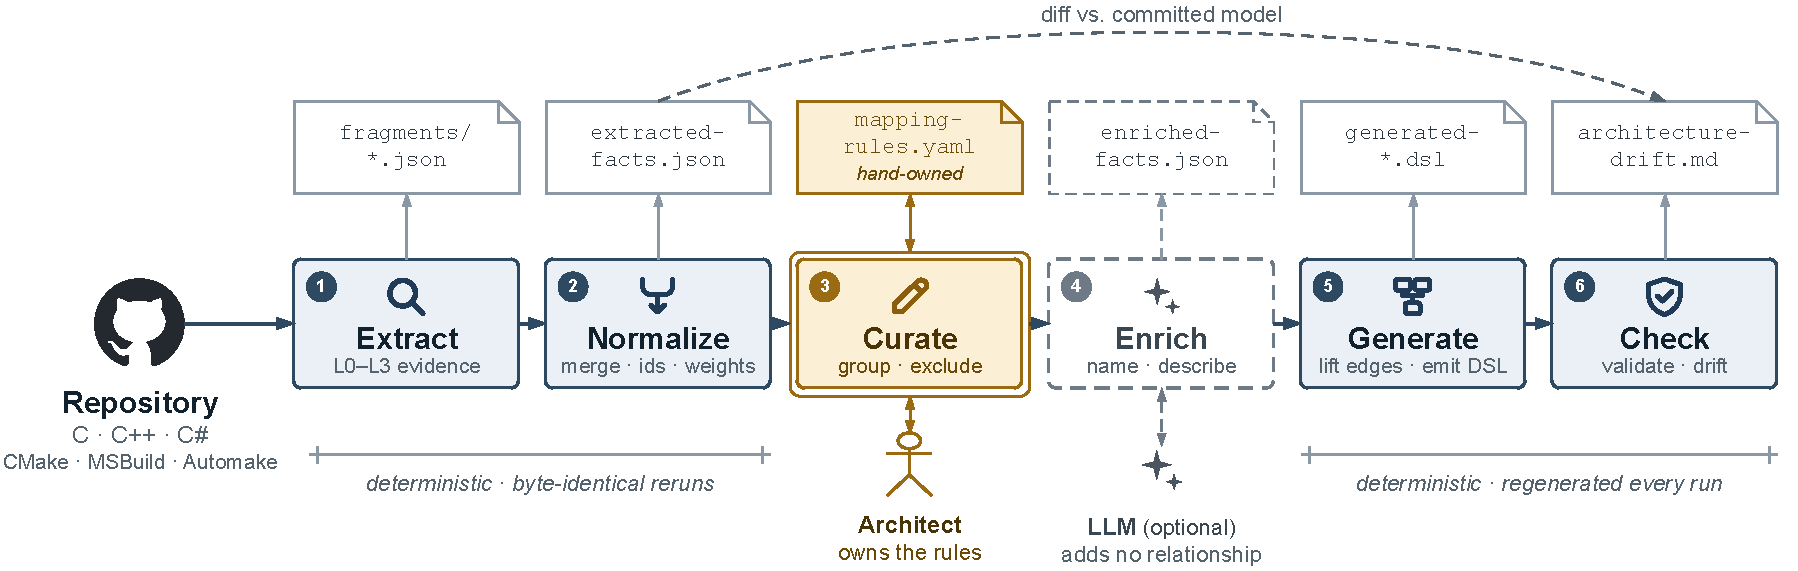
\includegraphics[width=0.9\textwidth]{figures-hand/pipeline.pdf}
  \caption{The pipeline. Blue stages are deterministic and regenerate byte-identically; the one
  human gate is stage~3, driven by the hand-owned mapping-rules file (amber, double border); the
  optional LLM stage (dashed) may only name and describe elements the evidence already contains,
  never add, remove, or move a relationship. Each stage writes the artifact above it; stage~6
  validates the model, checks the layering rules, and diffs freshly extracted facts against the
  committed model.}
  \label{fig:pipeline}
\end{figure*}
\section{Approach}
\label{sec:approach}

%% Revised 2026-08-30 against the GPT-5.6-Sol review and tightened for the page budget: module
%% (development) view scoped (6.1); "source of truth" -> primary evidence (A.2); L0--L3 (A.1);
%% LLM stage one paragraph, tested invariants stated here (4.6/A.7). Design constants are
%% literals on purpose. 2026-09-13 shortening pass (response plan §13, M6): the per-idiom extractor
%% detail added for the second review's point 5 keeps its substance (evaluated vs. static, what
%% each misses) and sends the target-type / alias / imported / partial handling and the generated
%% bash model figure (owner decision) to the TR.
%% 2026-09-13 readability pass: long sentences split, §III.A split into two paragraphs; no content change.


\tool{} turns a C/C++ or C\#\ repository into a governed model of its \emph{module view}: the
development-time decomposition into build targets and projects, and the compile-time dependencies
between them (link, include, symbol, and project references). It is rendered in the C4
notation~\cite{brown2026c4} of the Structurizr DSL~\cite{structurizrdsl}, the notation architects
keep. Using C4's container level for build units is a deliberate adaptation (a static library is
not a deployable unit): Structurizr's styles, drill-down, and tooling attach to that level. We
claim no runtime or deployment semantics.
Figure~\ref{fig:pipeline} shows the six stages. Three invariants shape every design decision: the
build graph is the primary structural evidence, which source-level evidence refines but never
replaces (\S\ref{sec:evidence}); a language model may name and describe elements but cannot add,
remove, or move a relationship (\S\ref{sec:enrich}); and the same inputs regenerate the same bytes
(\S\ref{sec:generate}). The first is a claim the study tests; the other two are held by tests on
every change.
% (a provider that invents a relationship is rejected; two runs must be byte-identical).

\subsection{Evidence extraction: build graph first}
\label{sec:evidence}

We distinguish evaluated from static extraction. For CMake the pipeline configures the project
once (Ninja generator) and reads CMake's File API codemodel of that configured tree: targets of
every type and the link dependencies as CMake evaluated them, generator expressions and conditions
included. For .NET the L0 layer is a static parse of \texttt{.sln} and \texttt{.csproj} files that
takes every \texttt{<ProjectReference>} regardless of MSBuild conditions and follows no import;
the Roslyn layer then loads the solution, an evaluated view. MSBuild C++ projects and automake or
hand-written \texttt{Makefile.in} are parsed statically: imports, property expansion, and
conditionals are not evaluated, so a conditional reference is over-approximated and one reachable
only through an import is missed (per-idiom detail and the graphviz cross-check of CMake edges:
\trExtract{}).

These declared dependencies form evidence layer L0; package references form L1; L2 adds the
\texttt{\#include} graph (Doxygen XML or \texttt{clang-scan-deps}) and Roslyn symbol references;
L3 (P/Invoke interop, deployment descriptors) is not evaluated here. Every extractor writes an
independent JSON fragment and degrades gracefully: without its toolchain it records a coverage
warning and an empty fragment. Per-layer coverage travels with the facts; its L0 denominator is
the first-party target set. A few \emph{refinement} extractors add no structure, only tags from
conventions the source declares (\texttt{.csproj} SDK role, OrchardCore module category, plugin
naming) for curation to group on. Declared dependencies are evidence, not truth (test, packaging,
and obsolete relations; missed runtime coupling), so curation excludes test and vendored targets
and the check stage reports a declared dependency no source file exercises.

\subsection{The fact model}
\label{sec:factmodel}

Normalization merges all fragments into one plain-JSON \emph{architecture fact model}, the
schema-validated contract between the extractors and any generator. Elements carry
content-independent identifiers (CMake target identity, project path), never a display name, so
a rename leaves identity intact and a move is pinned with an explicit alias. Evidence lists
citing the literal build-file
line, include, or symbol are concatenated and de-duplicated, and every derived quantity is
recomputed from the merged evidence. \emph{Weight}, the edge intensity the threshold of
\S\ref{sec:curate} reads, is a deterministic sum over that evidence, its constants pinned in one
module: 5 per declared link or project reference, 1 per package
reference, an include item's file count capped at 10 so one chatty header cannot dominate, a
symbol-use item's count, and 5 per P/Invoke. \emph{Confidence} is computed orthogonally (low for
a declared link no source exercises). Every edge with L0 evidence is marked \emph{declared}, no
relationship exists without evidence, all lists are canonically ordered, and a
provenance-stripped hash of the model is the idempotency and drift key.

\subsection{Curation: rules as code behind a human gate}
\label{sec:curate}

A dependency graph is the wrong altitude for an architecture diagram, so a curation step maps many
build targets onto fewer containers through a hand-reviewed \texttt{mapping-rules.yaml} in a
propose--review--lock loop. \cli~\texttt{propose} drafts rules from explainable heuristics
(layout, namespace roots, target-name patterns, edge weight, the convention tags above), and the
architect accepts or edits them in the YAML or a tree editor. Once committed, every run is
deterministic until a target appears that no rule covers; it is rendered as its own container
tagged \texttt{needs-curation}, never guessed. Rules group members by identifier, path
glob, or tag; exclude test, generated, and vendored targets; pin names; and set the significance
threshold (default 3) for non-declared edges only. A declared dependency is never dropped by
weight, only by explicit exclusion. The curator chooses the boxes; the evidence draws the arrows.

\subsection{Enrichment: language, not structure}
\label{sec:enrich}

The LLM stage is off by default and never runs in CI; the evaluated technique is the deterministic
one. Its input is the curated fact model after a redaction pass and a field whitelist:
identifiers, types, top dependencies, and documentation snippets of at most 280 characters, never
a source file. Its output is validated against a JSON schema and a referential-integrity check
that rejects any element or relationship the facts do not already contain, so its structural
footprint is zero by construction.

\subsection{Generation and governance}
\label{sec:generate}

The generator lifts target-to-target edges to container-to-container edges, merging parallel
and dropping intra-container ones, and emits two machine-owned DSL fragments that the
hand-owned \texttt{workspace.dsl} includes. Views, styles, and saved layout are scaffolded once,
and stable DSL identifiers let Structurizr re-attach saved positions after a regeneration (one
generated model with its evidence traced: \trExtract{}). The check stage diffs freshly extracted facts against the committed model and reports new and
vanished targets and edges, suspected renames, declared-but-unused dependencies, and violations of
forbidden container-to-container edges from a layering-rules file. Three stopping rules keep it
from crying wolf. A disappearance is drift only if the evidence layer that produced it was
extracted in both runs, otherwise a labelled coverage gap. Below 80\,\% first-party L0 coverage,
or with no first-party target extracted at all, the report is advisory and stops gating. A layering check over degraded evidence answers \texttt{UNVERIFIED} rather than passing.
Drift is always a report, never an automatic edit.

\section{Study Design}
\label{sec:design}

%% Revised 2026-08-30 against the GPT-5.6-Sol review (plans/2026-08-30-saner-review-response-plan.md)
%% and tightened for the page budget. Numbers are macros only.
%% 2026-09-13 shortening pass (response plan §13): the terminology paragraph is the shared
%% latex/shared/terms.tex (also used by the TR; captions cite it as \S\ref{sec:design}); M5/M7
%% send the full inferential machinery, the metric definitions and the entity-ownership
%% tie-breaks to the TR; caveats stated here are not restated in §V/§VI.
%% 2026-09-13 readability pass: long sentences split, §IV.D split into two paragraphs; no content change.

The study is built so the two-regime thesis of \S\ref{sec:intro} can fail.
\emph{Recoverability} (RQ1--RQ3) asks how much of a system's module structure is recoverable from
build and dependency evidence alone, and where that breaks down. \emph{Expression and governance}
(RQ4--RQ7) asks whether, where recovery fails, a human-in-the-loop pipeline keeps the expressed
architecture stable, checkable, and affordable in a way autonomous SAR does not.
\textbf{RQ1:} how much does build evidence alone recover, can that be diagnosed without a
reference, and where is human input needed? The autonomous rows are the \emph{no-curation floor}
and the \emph{auto-propose draft} (defined below). \textbf{RQ2:} given the same dependency input,
do the autonomous rows match classical SAR and a controlled LLM baseline, and how far does
curation move the score? \textbf{RQ3:} which design choices contribute, at the operating
configuration and at the extremes? \textbf{RQ4:} are outputs identical across reruns, and does
the decomposition survive code change? \textbf{RQ5:} does drift detection report seeded and real
change at an acceptable false-finding cost, and fail honestly when evidence goes missing?
\textbf{RQ6:} how do runtime and memory scale against the pipeline's own budget? \textbf{RQ7:}
where recovery fails, how close does a reference-blind curator get to the reference, at what
effort, and how does that compare with the agreement between two reference authors? The plan's
RQ identifiers are mapped in the artifact.

%% The shared terminology paragraph (was the boxed Table I until 2026-09-13; folded into prose
%% for the page budget, response plan section 13 status). The legend the table captions used to
%% carry lives here once; captions reference \S\ref{sec:design} (the enclosing section: IV in the
%% paper, 1 in the TR, which labels its scope section sec:design too) instead of restating it.
%% SHARED between main.tex and tr.tex: it must not reference a label that exists in only one of
%% the two documents. Hand-owned: definitions, not data.
\paragraph{Terminology.}
Three \emph{rows} recur in every table: the \emph{floor} (autonomous: every scored entity in its
owning build target, no curation), the \emph{propose} draft (autonomous: the tool's heuristic rule
draft accepted verbatim), and the \emph{curated} model (the committed hand rules applied). A
\emph{detection} number scores autonomous recovery, an \emph{expression} number what a human
expressed under evidence constraints; the two are never compared inferentially, and only detection
numbers support a recovery claim. Curation provenance (Cur.): \emph{sighted} = reference in view,
so the score is an oracle-assisted upper bound, never evidence against an autonomous technique;
\emph{assisted} = LLM-assisted from names and directories, the reference mapping not consulted;
\emph{blind} = reference-blind curator (RQ7); \emph{none} = curated model identical to the floor.
Reference grades (Ref) and the \emph{all-common} projection are defined in
\S\ref{sec:corpus} and \S\ref{sec:baselines}.

Curation sets the very partition the metrics score, so a curated score compares assisted with
unassisted recovery and says nothing about autonomous recovery. Every detection claim rests on
the two autonomous rows; the non-circular curated numbers come from the reference-blind
curations (RQ7; Squidex's only curated model). Three of the four C\#\ curations
were authored with the reference in view, and P-1's with the diagram its reference was
reconciled from (Table~\ref{tab:corpus}).

\subsection{Subject corpus and references}
\label{sec:corpus}

\textbf{Tier-A} (Nine systems: five C/C++, four C\#) carries
a reference architecture and drives RQ1--RQ3 and RQ7 (Table~\ref{tab:corpus}); \textbf{Tier-B}
(\rqSevenSystems{} systems, containing Tier-A) needs none and drives RQ4--RQ6. The anonymized
industrial system, \textbf{P-1} in the tables, sits outside both tiers: its metrics corroborate
the open-source results but are not replicable. Tier-B spans three orders of magnitude in KLOC and
four build idioms (CMake, .NET SDK, MSBuild-C++, automake or hand-written \texttt{Makefile.in}),
which co-vary with language here (\S\ref{sec:threats}). Every system is pinned to a commit;
nopCommerce's source (license) and libxml2's reference (third-party) stay out of our package,
their measurements in. \textbf{GT-pub} adopts a published mapping verbatim. \textbf{GT-doc} is transcribed from the project's own documentation by two
people independently, then reconciled. For \textbf{GT-exp}, two architects map entities to
components blind to the pipeline output; we report their agreement (\S\ref{sec:metrics}), resolve
by discussion, and flag $\kappa<0.6$ as lower-confidence. abseil is the exception: a single
rater applied its documented one-library-per-directory layout, so no agreement is reported. No
system's curator authors its reference. Table~\ref{tab:corpus} records each curation's provenance (attested; overlay and
reference commit dates in the artifact).

\subsection{Baselines, their inputs, and fairness controls}
\label{sec:baselines}

We compare against \rqTwoBaselineCount{} classical SAR and na\"ive baselines plus a controlled
LLM-recovery baseline. The semantic and agentic lines of \S\ref{sec:background} are discussed, not
run: SARIF's only release is a closed Linux binary without C\#\ support, FCA is an unlicensed
MATLAB script, and the four most recent comparative evaluations themselves take this classical
set as their baselines~\cite{zhang2023sarif,zhao2026semarc,ding2026ssar,zhang2026semref}. The
classical set is ACDC~\cite{acdc}, ARC~\cite{arc}, WCA~\cite{wca}, and LIMBO~\cite{limbo}
(\S\ref{sec:background}), all run through the
\textsc{Arcade} workbench~\cite{arcade}, which also supplies the MoJoFM and a2a implementations
(c2c is not reported). Two na\"ive lower
bounds, directory-tree clustering and connected components, complete the set. The
\textbf{LLM-recovery baseline} stands for the LLM-centric line~\cite{archagent}: a reasoning-tier
model (\texttt{gpt-5.6-sol}, pinned) receives the exported graph, one line of repository
metadata (the system's name and language), and the same $k$ as ARC under one prompt asking for a JSON entity-to-cluster map, at
default sampling and a 180\,k-token input budget; five reruns on \rqTwoLlmSystemsRan{} systems at
most \$\rqTwoLlmCostMaxUsd{} per system, mean and spread reported, prompt and replies in the
artifact (\trInputs{}).

\paragraph{What each technique receives.} One dependency graph per system, exported once as RSF at
the scored granularity, feeds every technique: at project granularity (C\#) every relationship
kind between first-party projects as one unweighted edge set; at file granularity (C++) the
\texttt{\#include} graph, declared link edges never projected onto files. ACDC and
\texttt{cc} see the edges only; \texttt{dir} sees entity paths; WCA and LIMBO also receive $k$,
the reference cluster count, as their stopping point; ARC receives $k$ and each entity's source
text; the LLM receives the graph, the metadata line, and $k$. $k$ is an oracle hint no pipeline
row gets. The pipeline's autonomous rows instead know each entity's \emph{owning build target},
the signal under test, which no baseline receives in any form. A file belongs to the target whose
source list names it, else to the target owning the longest directory prefix; files no target
claims stay unclustered and count against the floor (\trInputs{}). RQ2 therefore compares the
whole pipeline with clustering the same edges, not two algorithms on identical information. No
baseline receives convention tags, documentation, or mapping rules; the curated row does, hence
its expression label.

\paragraph{Fairness controls, fixed before scoring.} One granularity per comparison (file for
C++, project for C\#), the pipeline's per-entity cluster induced via
\texttt{entity}$\to$\texttt{target}$\to$\texttt{container}; the same reference and metric
implementation for every technique; default parameters; and an \emph{all-common} entity
projection on which every number in Tables~\ref{tab:rq1} and~\ref{tab:rq2} is scored, floor and
propose included. ARC abstains on low-text files; it is scored on its own covered subset and kept
outside every paired test. A technique that does not complete is reported as missing. \emph{Lead}
is defined, not asserted: a row leads a system when it strictly exceeds every all-common classical
baseline (ACDC, WCA, LIMBO, \texttt{dir}, \texttt{cc}) on that metric; wins-or-ties and wins
against all displayed methods are reported beside it. The \emph{recovery bands} are post hoc:
recovered at MoJoFM $\ge\rqTwoRecoveredMin{}$, the score the reference-free diagnostic of
\S\ref{sec:metrics} is checked against, failed below \rqTwoFailedBelow{}, partial between.

\subsection{Ablations and blind curation}
\label{sec:ablation}

Eight axes toggle independently from the full configuration, paired per system on Tier-A: A1 caps
the evidence ladder at L0, L1, or L2; A2 walks the curation rungs (floor, single heuristics, the
auto-propose draft, hand rules); A3 sweeps the weight threshold; A4 toggles visibility
down-weighting; A5 switches off the never-drop-declared rule at the operating threshold and above;
A6 reads the RQ2 LLM-recovery runs as the LLM-does-structure arm; A7 toggles LLM naming; A8 measures stability under code
change. A frozen \texttt{mapping-rules.yaml} per system holds curation constant.

The blind-curation experiment (RQ7) yields the curation-vs-reference numbers that are not
circular. Its protocol, roles, and stopping rule were written into the plan before any session
and are unchanged since (dated commit history and signed attestations in the artifact; no external
registry). It ran on two C\#\ systems with four researchers in disjoint roles: eShop, whose
documented reference two raters re-derived independently as the leakage check against the sighted
curation, and Squidex, whose reference the raters built. Reference authors R$_1$ and R$_2$ work
from code and project docs. A curator C, who is neither, authors the mapping rules blind to the
reference, to R's mappings, and to any score, using the repository, docs, \cli~\texttt{propose}
draft, build facts, and GUI. C stops when the model is review-complete by their own judgment;
the harness logs the edit trace and wall-clock. Each system yields detection rows (the floor, the
best all-common technique), the expression row (the blind curator against the reference), and the
R$_1$-vs-R$_2$ agreement, an \emph{inter-rater baseline} that bounds nothing about a third
partition.

\subsection{Metrics and analysis}
\label{sec:metrics}

We lead with a2a~\cite{le2015a2a} and report MoJoFM~\cite{mojofm} second. MoJoFM rewards matching
the reference's cluster count, and a2a charges for the sprawl that produces, which is why the
na\"ive \texttt{dir} baseline beats the pipeline on MoJoFM on directory-aligned C++ but loses on
a2a. At a reviewer's request we add, post hoc and descriptively, the adjusted Rand index (ARI,
$\times$100), chance-corrected and charging over-splitting in full~\cite{zhang2023sarif}, and the
\emph{nested share}, the fraction of a partition's clusters lying inside one reference cluster,
which tells over-splitting from misgrouping. The inferential tests stay on MoJoFM and a2a.
\emph{Container-edge F1} scores the lifted container edges against the reference's own edge set
after a greedy label alignment; it is curation-constrained, not curation-proof, because the
grouping fixes which edges become intra-container. Inter-rater agreement is reported label-free
(ARI, normalized mutual information, and Cohen's $\kappa$ after Hungarian label matching), because
a raw label-match $\kappa$ measures wording. The raw $\kappa$ stays beside them because the plan's
flag rule (raw $\kappa<0.6$ marks a low-confidence reference) is applied as written.

To diagnose ``the build graph carries the architecture'' \emph{without} a reference we compute,
from the extracted facts alone, the floor's \emph{unit ratio} (build units per scored entity;
1.0 = every entity its own unit), its \emph{largest-unit share}, and its TurboMQ over the exported
graph. The rule over them was selected on the same systems it separates, so beside Spearman's
$\rho$ with a bootstrap interval we report the threshold interval over which it keeps its
agreement and a leave-one-system-out re-selection (\trDiagnostic{}). Governance is measured by
byte-identical regeneration and survivor-partition agreement at 20\,\% turnover (RQ4). Drift
detection (RQ5; \trDrift{}) is measured by precision and recall against seeded build-file
mutations run through the whole pipeline, per mutation and per finding; by the suppression rate
under induced evidence degradation; by the outcome of every seeded finding when a change and
evidence loss coincide; and by the findings between consecutive real releases under rules held
constant across each pair, each labelled by two raters. Performance (RQ6) is per-stage
wall-clock and peak RSS.

Scripts and thresholds were committed before results were unblinded. Across techniques (RQ2) the
inferential tests admit autonomous rows only: a Friedman omnibus on MoJoFM and a2a over the
all-common techniques with the floor (and, separately, the propose draft) in place of the curated
row, then Nemenyi and Holm-corrected pairwise Wilcoxon signed-rank tests of that row against each
technique (\trStats{}). The curated row enters no inferential test; its omnibus is descriptive. Paired on/off comparisons (RQ3) use Wilcoxon
signed-rank with the matched-pairs rank-biserial $r$. Cliff's~$\delta$ is reserved for the one
between-group contrast (C++ vs.\ C\#\ floor); detection rates get Wilson intervals, the stopping
rules exact McNemar, and the diagnostic Spearman's $\rho$. With $N\le 5$ paired systems the
two-sided exact signed-rank $p$ cannot fall below $0.0625$, and at $N=6$ not below $0.0312$,
however large the effect, so effect sizes and per-system deltas carry the argument. Every statistic is a generated macro.

\section{Results}
\label{sec:results}

%% Revised 2026-08-30 against the GPT-5.6-Sol review and tightened for the page budget. Every
%% detection headline names an autonomous row; curated C# scores are upper bounds; "lead" is the
%% defined strict rule; post-hoc pairs reported; A5 read at the operating point; RQ6 gains the
%% combined and real-history arms; RQ9's R1-vs-R2 row is inter-rater agreement. Macros only.
%% 2026-09-13 shortening pass (response plan §13): every result stays; the diagnostic's
%% sensitivity intervals (M4), the full inferential detail (M5), the SARIF/FCA numbers (M10),
%% the per-operator, combined-loss and per-pair history drift tables (M1, M2), the
%% rater-agreement forensics and the effort table (M3, M8) moved to the TR, each replaced by its
%% compact form. The caveats the terms box / §IV / §VII carry are not restated here.
%% 2026-09-13 readability pass: the RQ2 and RQ7 paragraphs split into three each, long sentences
%% split; every macro, number, and citation unchanged.

\subsection{RQ1: Recoverability, diagnosed without the reference}
\label{sec:rq1}
%% GENERATED by analysis/make_tables.py from results.csv -- DO NOT EDIT BY HAND.
\begin{table*}[t]
  \centering
  \caption{Corpus, RQ1 fidelity, and the A1/A5 ablation columns (terms: \S\ref{sec:design}). \#Cl./\#Ent./\#Tgt.\ = reference clusters, scored entities, first-party targets; Best = best all-common classical baseline by MoJoFM; A1 = container edges at L0 $\to$ all layers; A5 = container edges the never-drop-declared rule saves at threshold 3 / 8. GT-diag = inception-era diagram, architect-reconciled (P-1 curated with that diagram in view); $^\ddagger$anonymized proprietary system, non-replicable, corroborating only (entity count bucketed). P-1 floor/propose: its A2 rungs. $^\S$Squidex's only curated model is its reference-blind RQ7 curation.}
  \label{tab:corpus}\label{tab:rq1}\label{tab:rq3}
  \footnotesize\setlength{\tabcolsep}{3pt}
  \begin{tabular}{@{}lllll rrr rr rr rr r rr@{}}
    \toprule
    & & & & & & & & \multicolumn{2}{c}{Floor} & \multicolumn{2}{c}{Propose} & \multicolumn{2}{c}{Curated} & Best & A1 & A5 \\
    \cmidrule(lr){9-10}\cmidrule(lr){11-12}\cmidrule(lr){13-14}
    System & Lang & Build & Ref & Cur. & \#Cl. & \#Ent. & \#Tgt. & a2a & MoJo & a2a & MoJo & a2a & MoJo & MoJo & edges & t3/t8 \\
    \midrule
    ITK & C++ & CMake & GT-pub & assisted & 13 & 7657 & 79 & 84.2 & 96.9 & 97.8 & 98.3 & 99.6 & 98.4 & 93.9 & 17$\to$23 & 0/5 \\
    abseil & C++ & CMake & GT-exp & assisted & 21 & 809 & 190 & 85.1 & 89.9 & 100.0 & 100.0 & 98.8 & 95.2 & 97.8 & 79$\to$83 & 0/45 \\
    OpenCV & C++ & CMake & GT-doc & assisted & 14 & 1087 & 24 & 100.0 & 100.0 & 87.0 & 48.3 & 100.0 & 100.0 & 92.1 & 9$\to$9 & 0/5 \\
    bash & C & Makefile.in & GT-pub & assisted & 14 & 373 & 49 & 97.7 & 91.9 & 95.3 & 82.7 & 98.1 & 93.2 & 91.9 & 8$\to$17 & 0/5 \\
    libxml2 & C & automake & GT-pub & none & 18 & 82 & 14 & 76.0 & 11.4 & 73.5 & 5.7 & 76.0 & 11.4 & 31.4 & 3$\to$3 & 0/3 \\
    eShop & C\# & .NET SDK & GT-doc & sighted & 9 & 19 & 19 & 80.8 & 33.3 & 73.3 & 0.0 & 88.9 & 66.7 & 33.3 & 30$\to$30 & 0/30 \\
    OrchardCore & C\# & .NET SDK & GT-doc & sighted & 34 & 207 & 207 & 67.6 & 11.6 & 91.1 & 69.5 & 91.7 & 72.1 & 47.4 & 70$\to$72 & 0/26 \\
    nopCommerce & C\# & .NET SDK & GT-doc & sighted & 17 & 37 & 37 & 80.2 & 37.5 & 89.6 & 71.9 & 90.2 & 71.9 & 46.9 & 16$\to$30 & 0/0 \\
    Squidex$^\S$ & C\# & .NET SDK & GT-exp & blind & 12 & 15 & 26 & 92.0 & 70.0 & 86.8 & 50.0 & 95.8 & 70.0 & 70.0 & -- & -- \\
    P-1$^\ddagger$ & C++ & -- & GT-diag & sighted & 28 & 50-100 & 52 & 93.7 & 96.9 & 81.2 & 24.5 & 100.0 & 100.0 & 91.3 & -- & -- \\
    \bottomrule
  \end{tabular}
\end{table*}

%% Tables II/III anchored here (2026-09-13): same float-deferral reason as Fig. 1.
%% GENERATED by analysis/make_tables.py from results.csv -- DO NOT EDIT BY HAND.
\begin{table*}[t]
  \centering
  \caption{RQ2: MoJoFM (top) and a2a (bottom) vs.\ the reference on the all-common projection, best per row in bold. Strict wins against the five all-common baselines: curated 6 of 9 systems on MoJoFM and 7 of 9 on a2a; floor 2 of 9 and 2 of 9; propose 4 of 9 and 4 of 9. $^\dagger$ARC on its own covered subset. $^\S$LLM, mean $\pm$ sd of five reruns; -- = refused or not run. $^\ddagger$Anonymized proprietary system, non-replicable, corroborating only. P-1 floor/propose: its A2 rungs.}
  \label{tab:rq2}
  \footnotesize\setlength{\tabcolsep}{4pt}
  \begin{tabular}{@{}lrrrrrrrrrr@{}}
    \toprule
    System & Floor & Prop. & Curated & ACDC & ARC$^\dagger$ & WCA & LIMBO & dir & cc & LLM$^\S$ \\
    \midrule
    ITK & 96.9 & 98.3 & \textbf{98.4} & 70.3 & 49.2 & -- & -- & 93.9 & 48.4 & -- \\
    abseil & 89.9 & \textbf{100.0} & 95.2 & 41.1 & 25.1 & 31.2 & 35.1 & 97.8 & 19.5 & 98.8$\pm$0.2 \\
    OpenCV & \textbf{100.0} & 48.3 & \textbf{100.0} & 81.7 & 28.7 & 25.9 & 46.9 & 92.1 & 25.4 & \textbf{100.0}$\pm$0.0 \\
    bash & 91.9 & 82.7 & \textbf{93.2} & 60.5 & 32.3 & 52.8 & 51.6 & 91.9 & 62.5 & 84.2$\pm$1.6 \\
    libxml2 & 11.4 & 5.7 & 11.4 & 20.0 & 36.9 & 31.4 & 28.6 & 5.7 & 25.7 & \textbf{62.8}$\pm$1.1 \\
    eShop & 33.3 & 0.0 & 66.7 & 6.7 & 33.3 & 20.0 & 26.7 & 33.3 & 6.7 & \textbf{86.7}$\pm$4.2 \\
    OrchardCore & 11.6 & 69.5 & \textbf{72.1} & 24.2 & 40.8 & 32.6 & 47.4 & 11.6 & 24.2 & 30.2$\pm$1.3 \\
    nopCommerce & 37.5 & \textbf{71.9} & \textbf{71.9} & 28.1 & 56.2 & 46.9 & 34.4 & 37.5 & 28.1 & 60.6$\pm$3.2 \\
    Squidex & 70.0 & 50.0 & 70.0 & 0.0 & 50.0 & 50.0 & 60.0 & 70.0 & 0.0 & \textbf{76.0}$\pm$13.6 \\
    P-1$^\ddagger$ & 96.9 & 24.5 & \textbf{100.0} & 64.7 & 16.1 & 12.9 & 22.5 & 91.3 & 12.3 & -- \\
    \midrule
    System (a2a) & Floor & Prop. & Curated & ACDC & ARC$^\dagger$ & WCA & LIMBO & dir & cc & LLM$^\S$ \\
    \midrule
    ITK & 84.2 & 97.8 & \textbf{99.6} & 73.2 & 81.3 & -- & -- & 80.4 & 85.5 & -- \\
    abseil & 85.1 & \textbf{100.0} & 98.8 & 83.0 & 81.9 & 82.8 & 81.5 & 90.0 & 79.9 & 97.6$\pm$0.1 \\
    OpenCV & \textbf{100.0} & 87.0 & \textbf{100.0} & 86.3 & 82.3 & 81.2 & 84.7 & 86.6 & 81.4 & \textbf{100.0}$\pm$0.0 \\
    bash & 97.7 & 95.3 & \textbf{98.1} & 80.7 & 84.0 & 89.0 & 85.1 & 97.0 & 90.5 & 92.6$\pm$0.2 \\
    libxml2 & 76.0 & 73.5 & 76.0 & 76.6 & 87.0 & 84.2 & 82.0 & 73.5 & 78.0 & \textbf{91.3}$\pm$0.3 \\
    eShop & 80.8 & 73.3 & 88.9 & 75.9 & 89.4 & 86.0 & 85.9 & 80.8 & 75.9 & \textbf{97.9}$\pm$0.7 \\
    OrchardCore & 67.6 & 91.1 & \textbf{91.7} & 80.2 & 85.1 & 82.0 & 83.6 & 67.6 & 79.0 & 81.8$\pm$0.5 \\
    nopCommerce & 80.2 & 89.6 & 90.2 & 76.5 & 90.1 & \textbf{90.7} & 87.8 & 80.2 & 76.5 & 84.2$\pm$12.3 \\
    Squidex & 92.0 & 86.8 & 95.8 & 69.8 & 88.4 & 88.4 & 93.0 & 92.0 & 69.8 & \textbf{96.1}$\pm$1.4 \\
    P-1$^\ddagger$ & 93.7 & 81.2 & \textbf{100.0} & 88.5 & 79.5 & 78.4 & 81.3 & 87.3 & 78.2 & -- \\
    \bottomrule
  \end{tabular}
\end{table*}

%% GENERATED by analysis/make_tables.py from results.csv -- DO NOT EDIT BY HAND.
\begin{table*}[t]
  \centering
  \caption{Cluster count $k$ (left; Ref = reference clusters; -- = not recorded) and post-hoc ARI ($\times$100, right; best per row in bold; $^\S$mean $\pm$ sd of the LLM reruns) of every partition in Tables~\ref{tab:rq1} and~\ref{tab:rq2}. $^\dagger$ARC on its own covered subset. $^\ddagger$Anonymized proprietary system, non-replicable, corroborating only. P-1 floor/propose: its A2 rungs.}
  \label{tab:rq2k}
  \scriptsize\setlength{\tabcolsep}{2.5pt}
  \begin{tabular}{@{}l r r r r r r r r r r@{}}
    \toprule
    System & Ref & Floor & Prop. & Cur. & ACDC & ARC$^\dagger$ & WCA & LIMBO & dir & cc \\
    \midrule
    ITK & 13 & 78 & 8 & 8 & 1034 & -- & -- & -- & 212 & 46 \\
    abseil & 21 & 90 & 15 & 14 & 27 & -- & 20 & 20 & 31 & 1 \\
    OpenCV & 14 & 14 & 2 & 14 & 108 & -- & 8 & 13 & 86 & 3 \\
    bash & 14 & 16 & 6 & 10 & 54 & 12 & 13 & 12 & 11 & 7 \\
    libxml2 & 18 & 3 & 1 & 3 & 4 & 13 & 10 & 9 & 1 & 2 \\
    eShop & 9 & 19 & 1 & 14 & 2 & -- & 8 & 7 & 19 & 2 \\
    OrchardCore & 34 & 201 & 20 & 16 & 13 & -- & 34 & 33 & 201 & 1 \\
    nopCommerce & 17 & 37 & 8 & 9 & 1 & -- & 17 & 16 & 37 & 1 \\
    Squidex & 12 & 13 & 6 & 10 & 1 & 7 & 7 & 9 & 13 & 1 \\
    P-1$^\ddagger$ & 28 & 49 & 6 & 27 & 52 & 13 & 2 & 18 & 86 & 1 \\
    \bottomrule
  \end{tabular}\hfill
  \begin{tabular}{@{}l r r r r r r r r r r@{}}
    \toprule
    System & Floor & Prop. & Cur. & ACDC & ARC$^\dagger$ & WCA & LIMBO & dir & cc & LLM$^\S$ \\
    \midrule
    ITK & 22.6 & 84.6 & \textbf{99.3} & 2.9 & -- & -- & -- & 11.1 & -6.6 & -- \\
    abseil & 44.1 & \textbf{100.0} & 93.5 & 9.5 & -- & 11.4 & 4.2 & 62.8 & 0.0 & 85.8$\pm$0.1 \\
    OpenCV & \textbf{100.0} & 26.9 & \textbf{100.0} & 32.6 & -- & -0.7 & 4.9 & 40.8 & -0.2 & \textbf{100.0}$\pm$0.0 \\
    bash & 85.7 & 73.0 & \textbf{86.4} & 16.3 & 3.6 & 18.9 & 15.2 & 78.8 & 38.0 & 57.6$\pm$1.9 \\
    libxml2 & 1.6 & 0.0 & 1.6 & 0.8 & -2.1 & 16.8 & 10.0 & 0.0 & 8.0 & \textbf{46.1}$\pm$1.0 \\
    eShop & 0.0 & 0.0 & 45.1 & -1.4 & -- & -0.7 & 1.5 & 0.0 & -1.4 & \textbf{75.2}$\pm$6.8 \\
    OrchardCore & 0.0 & 59.4 & \textbf{84.1} & -1.8 & -- & 3.5 & 10.2 & 0.0 & 0.0 & 2.3$\pm$0.4 \\
    nopCommerce & 0.0 & \textbf{86.8} & 64.6 & 0.0 & -- & 16.4 & 8.1 & 0.0 & 0.0 & 23.7$\pm$1.7 \\
    Squidex & 0.0 & 20.7 & 20.9 & 0.0 & 10.6 & 7.5 & 17.5 & 0.0 & 0.0 & \textbf{44.0}$\pm$20.0 \\
    \bottomrule
  \end{tabular}
\end{table*}


\begin{figure}[t]
  \centering
  \resizebox{0.9\columnwidth}{!}{% GENERATED by analysis/make_figures.py from stats.json -- DO NOT EDIT BY HAND.
\begin{tikzpicture}
  \draw[thick] (0,0) rectangle (6.4,4);
  \draw (0.963,0) -- (0.963,-0.09); \node[below,font=\footnotesize] at (0.963,-0.09) {0.02};
  \draw (2.237,0) -- (2.237,-0.09); \node[below,font=\footnotesize] at (2.237,-0.09) {0.05};
  \draw (3.2,0) -- (3.2,-0.09); \node[below,font=\footnotesize] at (3.2,-0.09) {0.1};
  \draw (4.163,0) -- (4.163,-0.09); \node[below,font=\footnotesize] at (4.163,-0.09) {0.2};
  \draw (5.437,0) -- (5.437,-0.09); \node[below,font=\footnotesize] at (5.437,-0.09) {0.5};
  \draw (6.4,0) -- (6.4,-0.09); \node[below,font=\footnotesize] at (6.4,-0.09) {1};
  \draw (0,0) -- (-0.09,0); \node[left,font=\footnotesize] at (-0.09,0) {0};
  \draw (0,0.8) -- (-0.09,0.8); \node[left,font=\footnotesize] at (-0.09,0.8) {20};
  \draw (0,1.6) -- (-0.09,1.6); \node[left,font=\footnotesize] at (-0.09,1.6) {40};
  \draw (0,2.4) -- (-0.09,2.4); \node[left,font=\footnotesize] at (-0.09,2.4) {60};
  \draw (0,3.2) -- (-0.09,3.2); \node[left,font=\footnotesize] at (-0.09,3.2) {80};
  \draw (0,4) -- (-0.09,4); \node[left,font=\footnotesize] at (-0.09,4) {100};
  \node[below,font=\small] at (3.2,-0.5) {unit ratio (build units / scored entities, log)};
  \node[rotate=90,font=\small] at (-0.95,2) {floor MoJoFM (all-common)};
  \draw[densely dashed,black!60] (4.473,0) -- (4.473,4);
  \node[anchor=south east,rotate=90,font=\tiny,black!60] at (4.473,1.2) {ratio $\le$ 0.25};
  \draw[densely dashed,black!60] (0,3.2) -- (6.4,3.2);
  \node[anchor=south west,font=\tiny,black!60] at (0.132,3.2) {recovered $\ge$ 80};
  \node[font=\footnotesize,black!55] at (2.237,2.48) {build-modular};
  \node[font=\footnotesize,black!55] at (5.29,2) {project-coarse};
  \fill (3.435,3.597) circle (2pt);
  \node[anchor=east,font=\tiny] at (3.365,3.597) {abseil};
  \fill (3.571,3.678) circle (2pt);
  \node[anchor=west,font=\tiny] at (3.641,3.618) {bash};
  \draw (6.4,1.333) circle (2pt);
  \node[anchor=east,font=\tiny] at (6.32,1.263) {eShop};
  \fill (0.526,3.874) circle (2pt);
  \node[anchor=west,font=\tiny] at (0.596,3.744) {ITK};
  \draw (4.425,0.457) circle (2pt);
  \node[anchor=east,font=\tiny] at (4.355,0.457) {libxml2 (largest unit 78\,\%)};
  \draw (6.4,1.5) circle (2pt);
  \node[anchor=east,font=\tiny] at (6.32,1.6) {nopCommerce};
  \fill (0.468,4) circle (2pt);
  \node[anchor=west,font=\tiny] at (0.538,3.96) {OpenCV};
  \draw (6.4,0.463) circle (2pt);
  \node[anchor=east,font=\tiny] at (6.32,0.463) {OrchardCore};
  \draw (6.4,2.8) circle (2pt);
  \node[anchor=east,font=\tiny] at (6.32,2.8) {Squidex};
\end{tikzpicture}
}
  \caption{The two-regime finding in one view: the autonomous floor's MoJoFM against the build
  graph's unit ratio, which alone needs no reference. Dashed: the post-hoc rule's ratio
  threshold (\rqAdequacyRatioMax{}) and the recovery threshold (\rqTwoRecoveredMin{}). Filled
  markers satisfy the rule; libxml2 fails it through the largest-unit-share clause, not the
  ratio.}
  \label{fig:regimes}
\end{figure}

Table~\ref{tab:rq1} reads as a diagnosis carried by its autonomous columns. On four of the five
C/C++ systems the no-curation floor already sits within a few MoJoFM points of the curated model
(C++ median \rqOneFloorCppMoJo{}). On the four C\#\ systems it does not (median
\rqOneFloorCsMoJo{}): at project granularity the floor \emph{is} the all-singletons partition,
identical to \texttt{dir}, and the curated number is the curator's grouping. The auto-propose
draft is not a reliable autonomous comparator: it recovers abseil exactly
(\rqOneProposeAbseilMoJo{}) but collapses OpenCV into two containers (\rqOneProposeOpencvMoJo{})
and eShop into one (\rqOneProposeEshopMoJo{}). libxml2 marks the boundary from within C++: one
library target gives the build graph nothing to report. a2a tells the other half: the floor's
fine targets sprawl against a 13-cluster reference (ITK floor a2a \rqOneFloorItkAtoA{}), which
curation repairs. ARI (Table~\ref{tab:rq2k}) charges that sprawl in full: the floor scores
\rqOneFloorItkAri{} on ITK and \rqOneFloorAbseilAri{} on abseil although \rqOneFloorItkNested{}\,\%
and \rqOneFloorAbseilNested{}\,\% of its clusters lie inside one reference cluster, a refinement
rather than a misgrouping; the propose draft's merging restores \rqOneProposeItkAri{} and
\rqOneProposeAbseilAri{}. On bash and OpenCV, whose target counts sit near the reference's, the
floor's ARI (\rqOneFloorBashAri{}, \rqOneFloorOpencvAri{}) agrees with MoJoFM. ``Recovers''
therefore means at the granularity of the build targets.

The regime can be read off the build graph without the reference. The floor's \emph{unit ratio}
counts the build units that own at least one scored entity over the scored entities (hence below
Table~\ref{tab:rq1}'s \#Tgt). Across the \rqAdequacyN{} scored systems it correlates with the
floor's MoJoFM at Spearman $\rho=\rqAdequacyRhoRatioMoJo{}$ (bootstrap 95\,\% interval
$[\rqAdequacyRhoCiLo{}, \rqAdequacyRhoCiHi{}]$; $\rqAdequacyRhoRatioAtoA{}$ with a2a) and its
TurboMQ at $\rho=\rqAdequacyRhoMqMoJo{}$. The post-hoc rule ``unit ratio
$\le\rqAdequacyRatioMax{}$ and largest-unit share $\le\rqAdequacyLargestMax{}$'' declares
\rqAdequacyAdequateCount{} systems build-modular (ITK, abseil, OpenCV, bash) and
\rqAdequacyInadequateCount{} not (every C\#\ system at ratio 1.0; libxml2's one library holds
\rqAdequacyLibxmlLargestShare{} of the files), and agrees with a floor MoJoFM of at least
\rqTwoRecoveredMin{} on \rqAdequacyRuleAgreement{} systems (Fig.~\ref{fig:regimes}). The
separation is not knife-edge: the ratio threshold can sit anywhere in
$[\rqAdequacyRatioIntervalLo{}, \rqAdequacyRatioIntervalHi{})$ without changing a call, but
re-selecting both thresholds leave-one-system-out predicts \rqAdequacyLooCorrect{} and misses
\rqAdequacyLooWrong{}, the one system the largest-unit clause exists for (intervals, the
ratio-only variant, Tier-B calls: \trDiagnostic{}). The rule is deliberately simple and a hypothesis for the extension corpus
(\S\ref{sec:threats}). It calls none of the \rqAdequacyTierBSystems{} unreferenced Tier-B
systems build-modular; fmt (\rqAdequacyFmtUnits{} CMake targets over \rqAdequacyFmtEntities{}
files) is the project-coarse C++ case the scored corpus lacks.

\subsection{RQ2: Comparison with classical SAR and an LLM baseline}
\label{sec:rq2}

Table~\ref{tab:rq2} gives every technique the same graph and reference on both metrics. Against
the five all-common classical baselines the floor leads strictly on \rqTwoFloorMoJoWins{} systems
by MoJoFM (\rqTwoFloorMoJoWinsOrTies{} with ties; on C\#\ floor and \texttt{dir} coincide) and on
\rqTwoFloorAtoAWins{} by a2a; the propose draft on \rqTwoProposeMoJoWins{} and
\rqTwoProposeAtoAWins{}. On C\#\ the classical techniques collapse into one or two blobs through
the shared building-block projects, and on libxml2 everything sits at the floor. The curated
model leads strictly on \rqTwoPipelineMoJoWins{} systems by MoJoFM and \rqTwoPipelineAtoAWins{} by
a2a against the classical set, and on \rqTwoPipelineMoJoWinsAll{} and \rqTwoPipelineAtoAWinsAll{}
against every displayed baseline including ARC and the LLM. On C\#\ that margin is curation,
sighted on three systems (Table~\ref{tab:corpus}).

Under the post-hoc ARI of Table~\ref{tab:rq2k} the picture sharpens rather than changes. No
classical technique exceeds \rqTwoSarAriMax{} (\rqTwoSarAriMaxWhere{}) on any system, and the
C\#\ classical cells sit at chance. The curated model leads on \rqTwoPipelineAriWins{} systems,
the propose draft on \rqTwoProposeAriWins{}, and the floor on \rqTwoFloorAriWins{}, its
over-splitting of the two finest build graphs now visible. On the autonomous rows no difference
reaches significance, which at $n=\rqTwoFriedmanFloorN{}$ speaks to power, not to equivalence.
The Friedman omnibus does not reject equality with the floor
(MoJoFM $p=\rqTwoFriedmanFloorP$, a2a $p=\rqTwoFriedmanFloorAtoAP$, $n=\rqTwoFriedmanFloorN$) or
with the propose draft ($p=\rqTwoFriedmanProposeP$ and \rqTwoFriedmanProposeAtoAP{}) in place of
the curated row, and no Holm-corrected pairwise Wilcoxon or Nemenyi comparison separates either
row from any technique (\trStats{}). The curated row's omnibus ($p=\rqTwoFriedmanP$; differs from
\rqTwoPosthocDiffers{} after correction) is descriptive only.

By the post-hoc bands no classical technique reaches the recovery threshold on any of the four
C\#\ systems: \rqTwoCsClassicalFailed{} of \rqTwoCsClassicalCells{} technique--system cells fail,
and the \rqTwoCsClassicalPartial{} partial ones (\rqTwoCsClassicalPartialList{}) stay far below
\rqTwoRecoveredMin{}. The LLM is the strongest autonomous comparator: it recovers
\rqTwoLlmCsRecovered{} (\rqOneLlmEshopMoJo{}), is partial on \rqTwoLlmCsPartial{}, fails on
\rqTwoLlmCsFailed{}, varies across reruns on Squidex (Table~\ref{tab:rq2}), and was not run on
ITK, whose file graph exceeds the input budget fourfold (no call was made). ARC did not
reproduce either~\cite{link2019value}. SARIF~\cite{zhang2023sarif} and FCA~\cite{teymourian2022fca}
published scores against the very references used here for bash, ITK, and libxml2
(\trPublished{}). Our floor sits above both on bash and ITK, and SARIF's own ACDC run sits below
our ACDC row, so our inputs do not handicap the baselines. On libxml2 SARIF's text-and-folder
fusion beats every structural partition we score.

\subsection{RQ3: Ablation}
\label{sec:rq3}

Ablations are paired per system (Table~\ref{tab:rq1}). \emph{Curation (A2):} on the all-common
set curation adds \rqThreeCurationLiftCpp{} MoJoFM points on C++ and \rqThreeCurationLiftCs{} on
C\#\ (paired $r=\rqThreeCurationRankBiserialCs{}$, $p=\rqThreeCurationWilcoxonP{}$; the two
language groups' floors differ with Cliff's $\delta=\rqThreeFloorCliffsCppVsCs{}$).
\emph{Evidence layers (A1):} L0 alone yields
most container edges and the symbol layer the remainder (per layer: \trAblation{}).
\emph{Declared dependencies never dropped (A5):} at the default threshold of 3 the rule saves
\rqThreeAfiveOperatingEdgesSaved{} edges on \rqThreeAfiveOperatingSystemsChecked{} systems,
because every declared dependency clears the bar on its base weight. At 8, where a curator might
silence noisy include edges, a scalar filter cuts declared edges it cannot tell from noise,
removing \rqThreeAfiveEshopEdgesSaved{} of eShop's container edges (edge counts move on
\rqThreeAfiveWilcoxonN{} systems, paired $r=\rqThreeAfiveRankBiserial{}$,
$p=\rqThreeAfiveWilcoxonP{}$; reference recall falls by \rqThreeAfiveRefRecallDropList{} on the
\rqThreeAfiveRefRecallSystems{} systems where it is scored, too few to test). Thresholding (A3)
barely moves the edge set at the operating point and visibility down-weighting (A4) is inert.
\emph{Names, never structure (A6, A7):} read as the LLM-does-structure arm, the RQ2 LLM runs
recover a competitive partition on small systems and beat the curated model on
\rqThreeSixLlmGtPipelineList{}. But the deterministic pipeline matches or beats them on
\rqThreeSixPipelineGeLlm{} of the systems they completed (median LLM MoJoFM
\rqThreeSixLlmMedianMoJo{}), and ITK did not fit one prompt. An adversarial provider that renames every
element perturbs \rqThreeSevenMaxStructuralDelta{} relationships on
\rqThreeSevenSystemsChecked{} systems, confirming the invariant of \S\ref{sec:enrich}.

\subsection{RQ4: Reproducibility and stability}
\label{sec:rq5}

Byte-identical regeneration is a tested invariant (\S\ref{sec:generate}), the contrast with ARC and
the LLM baseline. What we measure is survivor-partition agreement under code change (A8). After
20\,\% entity turnover the per-entity rules keep every surviving entity in its cluster
(\rqFivePipelineChurn{} on all eight systems), as does \texttt{dir} (\rqFiveDirChurnMedian{}),
whereas ACDC, a global optimiser, reshuffles survivors on every system (median
\rqFiveAcdcChurnMedian{}, down to \rqFiveAcdcChurnWorst{} on abseil). Rules bind identities rather
than graph optima, so the contrast is one of semantics, not of correctness: a frozen ACDC
partition would keep its survivors too, but assigns nothing to new entities and carries no
evidence. A8 does not say the model is still \emph{right} later: new targets surface as
\texttt{needs-curation} singletons for the human, which \S\ref{sec:rq6} counts on real history.

\subsection{RQ5: Drift detection and governance}
\label{sec:rq6}

\paragraph{Seeded mutations and degradation (correctness).} We injected \rqSixMutationCount{}
labelled changes (\rqSixOperatorCount{} operators: add and remove a dependency; add, remove,
rename, and merge a target) into the \emph{build files} of checkout copies of
\rqSixMutationSystems{} systems across three build idioms. We ran the whole pipeline on each and
scored the report against the label, one finding per vanished or new target, edge, rename, or
violation. The report covered \rqSixMutationsDetected{} mutations fully, with precision
\rqSixPrecision{}, recall \rqSixRecall{}, \rqSixFpPerPr{} false findings per simulated pull
request, renames classified as renames (accuracy \rqSixRenameAccuracy{}), and a one-line alias
pin silencing the drift in \rqSixAliasSurvival{} pinned reruns (per operator: \trDrift{}).
Inducing evidence degradation on the \rqSixDegradationSystems{} systems scored before Squidex
joined (semantic toolchain lost; 10\,\% and 30\,\% of targets starved of L0 evidence; build-graph
extractor lost) produces \rqSixWouldBeFalse{} would-be-false ``disappeared'' findings, of which
the stopping rules reclassify all of them as labelled coverage gaps (suppression rate
\rqSixSuppressionRate{}), where a
coverage-naive differ reports every one as change (exact McNemar $p\rqSixMcNemarP$).

\paragraph{Change and evidence loss at once.} Neither arm tests that degradation never hides
erosion, so we replayed the \rqSixCombMutations{} mutations on \rqSixCombSystems{} systems
with each degradation mode induced on the mutated run, plus an adversarial mode that starves
exactly the targets the mutation touches, and classified, per mode, each of the
\rqSixCombFindings{} expected findings as named drift, coverage gap, advisory-only, or silent (\trDrift{}). Under
targeted starvation \rqSixCombStarveMutatedDrift{} are drift, \rqSixCombStarveMutatedGap{} gaps,
and \rqSixCombStarveMutatedAdvisory{} advisory only. The experiment also found a hole: with the
build-graph extractor lost entirely, an added or renamed target was reported nowhere and the run
was not even advisory (\rqSixCombPrefixSilentTotal{} silent findings in that mode), because an empty
first-party target set counted as fully covered. After changing that convention (nothing covered,
advisory), \rqSixCombSilentTotal{} silent findings remain, the \rqSixCombLoseLZeroAdvisory{}
former ones are advisory, and no mode produced a false finding. The claim survives in a weaker
form: erosion is never hidden, but under heavy evidence loss it is often visible only as a warning
that evidence dropped.

\paragraph{Real history.} We then ran the detector over \rqSixHistPairs{} consecutive release pairs
of \rqSixHistSystems{} systems (libxml2, nopCommerce, Squidex), fixed in advance rather than
selected by changelog, with the committed rules held constant across each pair (per pair:
\trDrift{}). The \rqSixHistCommits{} commits, \rqSixHistBuildCommits{} of them touching build
files, yielded \rqSixHistFindings{} findings and \rqSixHistCoverageGaps{} coverage gaps;
\rqSixHistPairsZero{} pairs with build-file churn produced none. Of the \rqSixHistNewTargets{} first-party targets the releases added, the rules left
\rqSixHistNewUnmapped{} unmapped, as expected: the Squidex and nopCommerce overlays post-date both
releases, and libxml2's predate them. Two raters labelled each finding independently: both
called \rqSixHistArchitectural{} architectural, \rqSixHistNonArchitectural{} non-architectural and
\rqSixHistNoise{} extraction noise, with raw agreement \rqSixHistLabelsAgree{} and pooled
Cohen's $\kappa$ of \rqSixHistLabelsKappa{}.

\subsection{RQ6: Performance and scalability}
\label{sec:rq7}

Across \rqSevenSystems{} systems spanning \rqSevenMinKloc{}--\rqSevenMaxKloc{}\,KLOC, the cold
end-to-end run (CMake configure, Doxygen, and Roslyn included) stays within the 30-minute budget
on \rqSevenColdBudget{} systems and the warm rerun within the 3-minute budget on
\rqSevenWarmBudget{} (median speedup \rqSevenMedianSpeedup$\times$; log--log slope
\rqSevenScalingSlope{} against KLOC; peak RSS \rqSevenMaxPeakRssGb{}\,GB; per system:
\trPerf{}). The exception is ITK: its cold run takes \rqSevenItkColdMin{} minutes,
\rqSevenItkDoxygenSharePct{}\,\% of it in Doxygen's XML pass, against \rqSevenItkWarmMin{} warm.
At this size the L2 layer misses the per-commit budget; an L0-only run would take about
\rqSevenItkLZeroImpliedMin{} minutes (an estimate, not a measurement).

\subsection{RQ7: Curation value under blinding}
\label{sec:rq9}
%% GENERATED by analysis/make_tables.py from results.csv -- DO NOT EDIT BY HAND.
\begin{table}[t]
  \centering
  \caption{RQ7 blind curation (terms: \S\ref{sec:design}; all-common projection; best SAR = best of ACDC/WCA/LIMBO, \texttt{dir} coinciding with the floor here). R$_1$ vs.\ R$_2$ = the reference authors' agreement, an inter-rater baseline; Edge-F1 = container-edge F1; $\kappa$ = raw Cohen's $\kappa$ on rater labels; confl. = rater clusters cutting a reference boundary; the consensus row is a sensitivity re-score, the second-curator row the curator-variance arm.}
  \label{tab:rq9}
  \footnotesize\setlength{\tabcolsep}{2.2pt}
  \begin{tabular}{@{}lll rrl@{}}
    \toprule
    System & Row & Kind & MoJo & a2a & Edge-F1\,/\,$\kappa$ \\
    \midrule
    eShop & no-curation floor & det. & 33.3 & 80.8 & -- \\
     & best SAR (LIMBO) & det. & 26.7 & 85.9 & -- \\
     & \textbf{blind curator} & expr. & \textbf{86.7} & \textbf{95.8} & 0.63 \\
     & \quad second blind curator (R-B) & expr. & 66.7 & 90.8 & 0.56 \\
     & \quad curator vs.\ curator agreement & agr. & 80.6 & 93.9 & ARI\,0.75 \\
     & \quad vs.\ consensus & expr. & 75.0 & 92.0 & 0.55 \\
     & R$_1$ vs.\ R$_2$ agreement & agr. & 66.5 & 89.7 & $\kappa$\,0.00; 0\,confl. \\
    \midrule
    Squidex & no-curation floor & det. & 70.0 & 92.0 & -- \\
     & best SAR (LIMBO) & det. & 60.0 & 93.0 & -- \\
     & \textbf{blind curator} & expr. & \textbf{70.0} & \textbf{95.8} & 0.67 \\
     & R$_1$ vs.\ R$_2$ agreement & agr. & 54.5 & 86.3 & $\kappa$\,0.39; 0\,confl. \\
    \bottomrule
  \end{tabular}
\end{table}


On both systems the reference-blind curator lands above every classical technique on a2a and
above ACDC, WCA, and LIMBO on MoJoFM (Table~\ref{tab:rq9}): \rqNineEshopCuratorMoJo{} MoJoFM on eShop and \rqNineSquidexCuratorMoJo{} on
Squidex (a2a \rqNineEshopCuratorAtoA{} and \rqNineSquidexCuratorAtoA{}; container-edge F1
\rqNineEshopCuratorEdgeFone{} and \rqNineSquidexCuratorEdgeFone{}), \rqNineEshopOverBestSarMoJo{}
and \rqNineSquidexOverBestSarMoJo{} points above the best of ACDC, WCA, and LIMBO. The
informative comparison is against the reference, which on eShop
both raters, who never saw it, re-derive at \rqNineEshopRaterRefMoJoMin{} MoJoFM or better
(aligned $\kappa\ge$\rqNineEshopRaterRefKappaAlignedMin{}): it is not one author's opinion, and
the curator is at least as close to it as its re-derivers.

The plan's raw-$\kappa$ flag fired on both systems (\rqNineEshopKappa{}, \rqNineSquidexKappa{}),
but raw $\kappa$ scores exact label match. Label-free, eShop's raters agree (aligned $\kappa$
\rqNineEshopKappaAligned{}) and Squidex's disagree (\rqNineSquidexKappaAligned{}). On both systems
not one rater cluster cuts across a reference boundary: the partitions nest, and every
disagreement is about altitude, where the projects' documentation is silent (\trCuration{}).
eShop's sighted curation scored \rqNineEshopNonBlindMoJo{}; the blind curator scores
\rqNineEshopLeakageDelta{} points \emph{higher}, so reference access is not what carried the
sighted score, though curator differences remain a confound. The raters' consensus sits at a
coarser altitude (\rqNineEshopCuratorVsConsensusMoJo{} against it) and is a sensitivity row, not
a second reference. On Squidex the raters settled on fine granularity
(\rqNineSquidexConsensusClusters{} clusters over 15 projects), so the singleton floor is strong
(\rqNineSquidexFloorMoJo{}) and ACDC, WCA, and LIMBO fall below it. On the all-common projection
(13 of 15 reference projects; two have no first-party dependency and are unseen by the edge-only
techniques) the curator ties the floor on MoJoFM and lifts a2a from \rqNineSquidexFloorAtoA{} to
\rqNineSquidexCuratorAtoA{}; on the full reference it scores
\rqNineSquidexCuratorFullRefMoJo{}/\rqNineSquidexCuratorFullRefAtoA{}.

Effort was \rqNineEshopMinutes{} minutes and \rqNineEshopOps{} editor operations for eShop,
\rqNineSquidexMinutes{} and \rqNineSquidexOps{} for Squidex, whose curator worked in two
sittings around a GUI defect in that packet and inspected projects several times eShop's
size. A second, equally blind eShop curator (\rqNineEshopSecondCuratorCode{}), the one
measurement of curator variance, took \rqNineEshopSecondCuratorMinutes{} minutes over two
sittings and scored \rqNineEshopSecondCuratorMoJo{} MoJoFM (a2a
\rqNineEshopSecondCuratorAtoA{}): above every classical technique but
\rqNineEshopCuratorMoJoSpread{} points below the first curator, the two agreeing at aligned
$\kappa$ \rqNineEshopCuratorPairKappaAligned{} (\trCuration{}). No curator kept a group from the
\cli~\texttt{propose} draft (\rqNineEshopProposeDerivedPct\% and
\rqNineSquidexProposeDerivedPct\%), the same null the propose row of Table~\ref{tab:rq1} shows.

\section{Discussion}
\label{sec:discussion}

%% Revised 2026-08-30 against the GPT-5.6-Sol review and tightened for the page budget.
%% 2026-09-13 shortening pass (response plan §13): guards that §IV / §VII carry are referenced,
%% not restated; numbers and rationale §V already gives are not repeated.
%% 2026-09-13 readability pass: long sentences split; no number or claim changed.

\paragraph{The build graph earns its place, with a caveat.} The build layer alone recovers most
container edges (A1), and the autonomous floor recovers the module decomposition of every
build-modular system without a model or a human, at the granularity of its build targets. That
granularity is a refinement of the reference, which ARI charges and curation coarsens (RQ1). The
never-drop-declared rule (A5) is inert at the operating threshold and decisive above it, where a
scalar filter cuts the very \texttt{<ProjectReference>} edges that carry C\#\ structure: a
guard, reported as one.

\paragraph{Two regimes, defined by the build graph.} The diagnosis needs no reference to compute,
but its validity is not yet established without one: the post-hoc rule agrees with the floor on
\rqAdequacyRuleAgreement{} systems and survives leave-one-out on \rqAdequacyLooCorrect{}
(\S\ref{sec:rq1}). Where the build system composes
many entities into few units, the floor scores a median MoJoFM of \rqOneFloorAdequateMoJo{} and
curation adds \rqThreeCurationLiftCpp{} points. Even \texttt{dir} is competitive on MoJoFM there,
so a2a (curated lead on \rqTwoPipelineAtoAWins{} systems) is the fairer headline. Where every
entity is its own unit, the floor is \rqOneFloorCsMoJo{}, no classical technique reaches the
recovery threshold (best all-common C\#\ median: \rqTwoCsBestAllCommonName{}
\rqTwoCsBestAllCommonMoJo{}; ARC \rqTwoArcCsMoJo{} on its own subset), and the recovered
decomposition is the curator's grouping, worth \rqThreeCurationLiftCs{} points. The boundary
coincides with the language line here because .NET projects sit at architectural altitude and
CMake targets below it; libxml2 (CMake) crosses it from the C++ side, and the diagnostic
calls fmt and Terminal project-coarse too, untested without a reference. The honest claim is not that the pipeline recovers C\#\
architecture but that it lets a human \emph{express} it under evidence constraints (RQ7).

\paragraph{Where the model belongs.} LLM-as-structure works on small systems but varied across
reruns on one, did not fit ITK in one prompt, and was not contamination-controlled (A6); the
zero-footprint invariant holds under an adversarial provider (A7). Evidence for structure and the model for language is where the LLM line is
converging~\cite{sathvika2026views,angermeir2026reproducibility}.

\paragraph{Governance is the differentiator, within limits.} What the paper establishes is
governed module-view reconstruction: build-target membership, a curated module decomposition, and
evidence-drawn dependencies, scored as partitions. 
%Relationship validity is measured only by
%container-edge F1 on two systems, and the usefulness of the document not at all. 
%Per-entity rules
%keep every survivor in place under 20\,\% turnover, as does \texttt{dir}, whereas a rerun of ACDC
%reshuffles them down to \rqFiveAcdcChurnWorst{} (RQ4; a property of the rules, not the
%correctness of the evolved model). 
Seeded mutations show the detector is correct; the combined
arm shows erosion is never hidden, though often visible only as a warning.

%; and the real-history
%arm shows how quiet release pairs are (\rqSixHistFindings{} findings over \rqSixHistCommits{}
%commits), where the false-finding claim lives. A practitioner needs no model: run the
%diagnostic; where build-modular, accept the floor and curate the sprawl; where project-coarse,
%curate and commit the rules (\S\ref{sec:rq9}). The industrial system behaves like the OSS C++
%corpus (floor \tierPMedianFloorMoJo{} MoJoFM, curated \tierPMedianMoJo{}; Table~\ref{tab:rq1}).

\section{Threats to Validity}
\label{sec:threats}

%% Revised 2026-08-30: every residual the response plan (§6) leaves to the extension is named here
%% in the words the rebuttal uses. 2026-09-13 (plan §13): this section is the ONE home of every
%% caveat the results sections used to restate; design facts §IV states are referenced, not
%% repeated. 2026-09-13 readability pass: long sentences split; no threat added or dropped.

\paragraph{Construct.} ``Correct decomposition'' is a judgement, and no metric here assesses
semantic validity with architects. What we recover is a development-time module view rendered in
C4 notation, not a runtime container model (\S\ref{sec:approach}). Both RQ7
references fell below the raw-$\kappa$ flag; label-free measures and the nesting count show the
disagreement is granularity (\S\ref{sec:rq9}). Container-edge F1 is
curation-constrained, not curation-proof. c2c and adjusted a2a are not reported. The recovery
bands and the adequacy thresholds are post-hoc reading labels, not established boundaries. The
build graph is extracted, not validated against an independent evaluated source: CMake's File
API is the configured project's own evaluated model, cross-checked against CMake's graphviz
output, and the MSBuild-C++, automake, and C\#\ L0 parses are static, so a consistently
extracted graph can be consistently incomplete.

\paragraph{Internal.} The committed curations were authored with an LLM assistant and, on three
C\#\ systems and P-1, with the reference in view (Table~\ref{tab:corpus}). Their scores are
oracle-assisted upper bounds (\S\ref{sec:design}; RQ7 bounds the leakage on eShop only). Two C\#\ references transcribe the projects' naming and manifest
conventions, which the refinement extractors also mine, so a rule keyed on the convention scores
near-perfectly by construction; that score is reported only as a labelled reconstruction ceiling.
OpenCV's GT-doc mirrors the CMake module list and abseil's GT-exp the one-library-per-directory
layout, so their floor scores carry the same convention overlap. The LLM baseline's prompt named
the system and used the real identifiers of publicly documented systems, so training-data
contamination is uncontrolled.
The regime claim is confounded by build technology, granularity, style, size, and reference
provenance, all co-varying with language here. The reference-free diagnostic separates the
build-graph property from the language, but it is post hoc, selected on the nine systems it
separates, with one of its two clauses carried by a single system (\S\ref{sec:rq1}): a
candidate diagnostic, not a validated predictor.

\paragraph{External.} Nine OSS  and one proprietary
system are not the industrial population, and the pipeline favours CMake. %
%; the MSBuild-C++ path has no Tier-A system and is never scored against a reference. 
RQ7 ran on two systems of 19 and 15 projects with three curators overall. Curator variance therefore rests on one pair
(\rqNineEshopCuratorMoJoSpread{} MoJoFM points apart), the
effort numbers are two measurements, and we claim nothing about larger C\#\ systems or manual
modelling.
%, whose comparator arm did not run: the governance advantages over hand
%modelling are stated as properties, not measured. 
Blinding removed copying and tuning, not the
priors of shared public documentation (\S\ref{sec:design}). The drift results are largely
construction-verified. The seeded and combined arms confirm correctness under evidence loss, and
the real-history arm covers \rqSixHistPairs{} release pairs of \rqSixHistSystems{} systems with a
handful of findings, under rules that post-date the releases on two of the three. The seeded
operators cover no splits or file moves, and on real history most changes are intended evolution,
so effectiveness on real erosion at scale is not established and the false-finding rate rests on
two raters' labels of \rqSixHistFindings{} findings.

\paragraph{Conclusion.} With $N\le 9$ paired systems we use non-parametric tests with Holm
correction, paired effect sizes, and per-system deltas. We fixed every threshold in the plan
before the data except the adequacy rule and the recovery bands; the plan's dated commit history
is the only record of that order, and no external registry was used. The RQ2 omnibus is reported
with and without the ninth system (\trStats{}).

\section{Conclusion}
\label{sec:conclusion}

%% Revised 2026-08-30: verdict phrased on the autonomous rows and the reference-free diagnostic;
%% the curator "reaches the ceiling" claim is gone; governance stated with its limits.
%% 2026-09-13 (plan §13): guards live in §VII; the verdict is stated once.
%% 2026-09-13 readability pass: one long sentence split; no claim changed.

The data support a narrower thesis than we started with. Where the build system composes many
entities into few units, a property computable before curating, the floor alone recovers the
module view, at the granularity of its build targets, without a model or a human. Where every
entity is its own unit, no classical technique reaches the recovery threshold, and the
contribution is expression. On two small systems, reference-blind curators produce a model that
regenerates byte-identically, survives code change without churn, and is drift-checked; erosion
is never silently hidden under evidence loss (though often visible only as a warning), and on
real history two raters agreed that \rqSixHistNoise{} of \rqSixHistFindings{} findings were
extraction noise. Future work: architect-assessment studies, runtime evidence, and more systems
per build idiom.


%% 2026-09-13 (owner decision, plan section 13 status): the URL only. What the package holds, the
%% four reproducibility classes of its rows (review O1), and the on-acceptance DOI/TR are in the
%% package README (baselines/make_review_artifact.py writes it), not here.
\paragraph{Data availability} Anonymized replication package, with the companion technical
report \TR{}: \texttt{<anonymous mirror URL>}.
\paragraph{Acknowledgments} Generative AI assisted manuscript editing and code implementation. All research methodology, analysis, and conclusions are the authors' contributions. 
 

\bibliographystyle{IEEEtran}
%% SCAFFOLD -- gated on \ifdraftbib (declared in the preamble). OFF since 2026-08-30: section II
%% cites for real, so the list holds only cited entries (a submission must not list uncited
%% references). Leave it off; references.bib may hold uncited spares for sections I/VI.
\ifdraftbib\nocite{*}\fi
\bibliography{references}

\end{document}
